% !TEX program = xelatex
\documentclass[a4paper,fontset=none]{ctexart}

\usepackage[a4paper,top=2.54cm,bottom=2.54cm,left=3.175cm,right=3.175cm]{geometry}
\usepackage{fontspec}
\usepackage{titlesec}
\usepackage{titletoc}
\usepackage{fancyhdr}
\usepackage{graphicx}
\usepackage{booktabs}
\usepackage{longtable}
\usepackage{tabularx}
\usepackage{array}
\usepackage{caption}
\usepackage{enumitem}
\usepackage{float}
\PassOptionsToPackage{pdfpagelabels=false}{hyperref}
\usepackage{hyperref}
\usepackage{xcolor}
\usepackage{setspace}
\usepackage{indentfirst}
\usepackage{tikz}
\usepackage{eso-pic}
\usetikzlibrary{arrows.meta,positioning,shapes.geometric}

\IfFontExistsTF{Times New Roman}{\setmainfont{Times New Roman}}{}
\IfFontExistsTF{Arial}{\setsansfont{Arial}}{}
% === 跨平台自动判断：宋体 ===
\IfFontExistsTF{SimSun}{
    % 如果电脑里有 SimSun (说明是 Windows)，就用这一套
    \setCJKmainfont{SimSun}
    \setCJKsansfont{SimSun}
    \newcommand{\SongBold}{\CJKfontspec[FakeBold=2.5]{SimSun}}
}{
    % 如果没有 SimSun (说明是 Mac)，就自动切换到 Songti SC
    \setCJKmainfont{Songti SC}
    \setCJKsansfont{Songti SC}
    \newcommand{\SongBold}{\CJKfontspec[FakeBold=2.5]{Songti SC}}
}

% === 跨平台自动判断：黑体 ===
\IfFontExistsTF{SimHei}{
    % 如果是 Windows 系统
    \newcommand{\HeiBold}{\CJKfontspec[FakeBold=2.5]{SimHei}}
}{
    % 如果是 Mac 系统
    \newcommand{\HeiBold}{\CJKfontspec[FakeBold=2.5]{Heiti SC}}
}

\makeatletter
\renewcommand\normalsize{%
  \@setfontsize\normalsize{12bp}{22bp}%
  \abovedisplayskip 12bp plus 2bp minus 5bp
  \abovedisplayshortskip 0bp plus 2bp
  \belowdisplayshortskip 8bp plus 2bp minus 4bp
  \belowdisplayskip \abovedisplayskip
  \let\@listi\@listI
}
\makeatother
\normalsize
\setlength{\parindent}{2em}
\setlength{\parskip}{0pt}
\setstretch{1}
\raggedbottom
\emergencystretch=2em

\titleformat{\section}
  {\raggedright\SongBold\fontsize{14bp}{22bp}\selectfont}
  {\chinese{section}、}
  {0pt}
  {}
\titlespacing*{\section}{0pt}{22bp}{22bp}

\titleformat{\subsection}
  {\raggedright\SongBold\fontsize{12bp}{22bp}\selectfont}
  {\hspace{2em}（\chinese{subsection}）}
  {0pt}
  {}
\titlespacing*{\subsection}{0pt}{22bp}{22bp}

\setcounter{secnumdepth}{2}
\setcounter{tocdepth}{2}
\renewcommand{\contentsname}{目\hspace{1em}录}
\titlecontents{section}
  [0pt]
  {\fontsize{12bp}{22bp}\selectfont}
  {\contentslabel{3em}}
  {}
  {\titlerule*[0.6pc]{.}\contentspage}
\titlecontents{subsection}
  [2em]
  {\fontsize{12bp}{22bp}\selectfont}
  {\contentslabel{4em}}
  {}
  {\titlerule*[0.6pc]{.}\contentspage}

\pagestyle{fancy}
\fancyhf{}
\renewcommand{\headrulewidth}{0pt}
\renewcommand{\footrulewidth}{0pt}
\cfoot{\thepage}

\captionsetup{
  font={normalsize},
  labelfont={normalsize},
  labelsep=space,
  justification=centering
}
\renewcommand{\arraystretch}{1.35}
\setlength{\tabcolsep}{6pt}

\setlist[itemize]{leftmargin=2em,itemsep=0pt,topsep=0pt,parsep=0pt,partopsep=0pt}
\setlist[enumerate]{leftmargin=2.5em,itemsep=0pt,topsep=0pt,parsep=0pt,partopsep=0pt}

\hypersetup{
  hidelinks,
  pdfauthor={},
  pdftitle={瞳伴——智能导盲陪行机器人商业计划书}
}

\newcommand{\ReportTitle}[1]{%
  \begin{center}
    \SongBold\fontsize{18bp}{22bp}\selectfont #1
  \end{center}
}

\newcounter{planitem}[subsection]
\renewcommand{\theplanitem}{\arabic{planitem}.}
\newcommand{\PlanItem}[1]{%
  \par
  \refstepcounter{planitem}%
  \indent\theplanitem\ #1
  \par
}

\begin{document}

\thispagestyle{empty}
\AddToShipoutPictureBG*{%
  \AtPageLowerLeft{%
    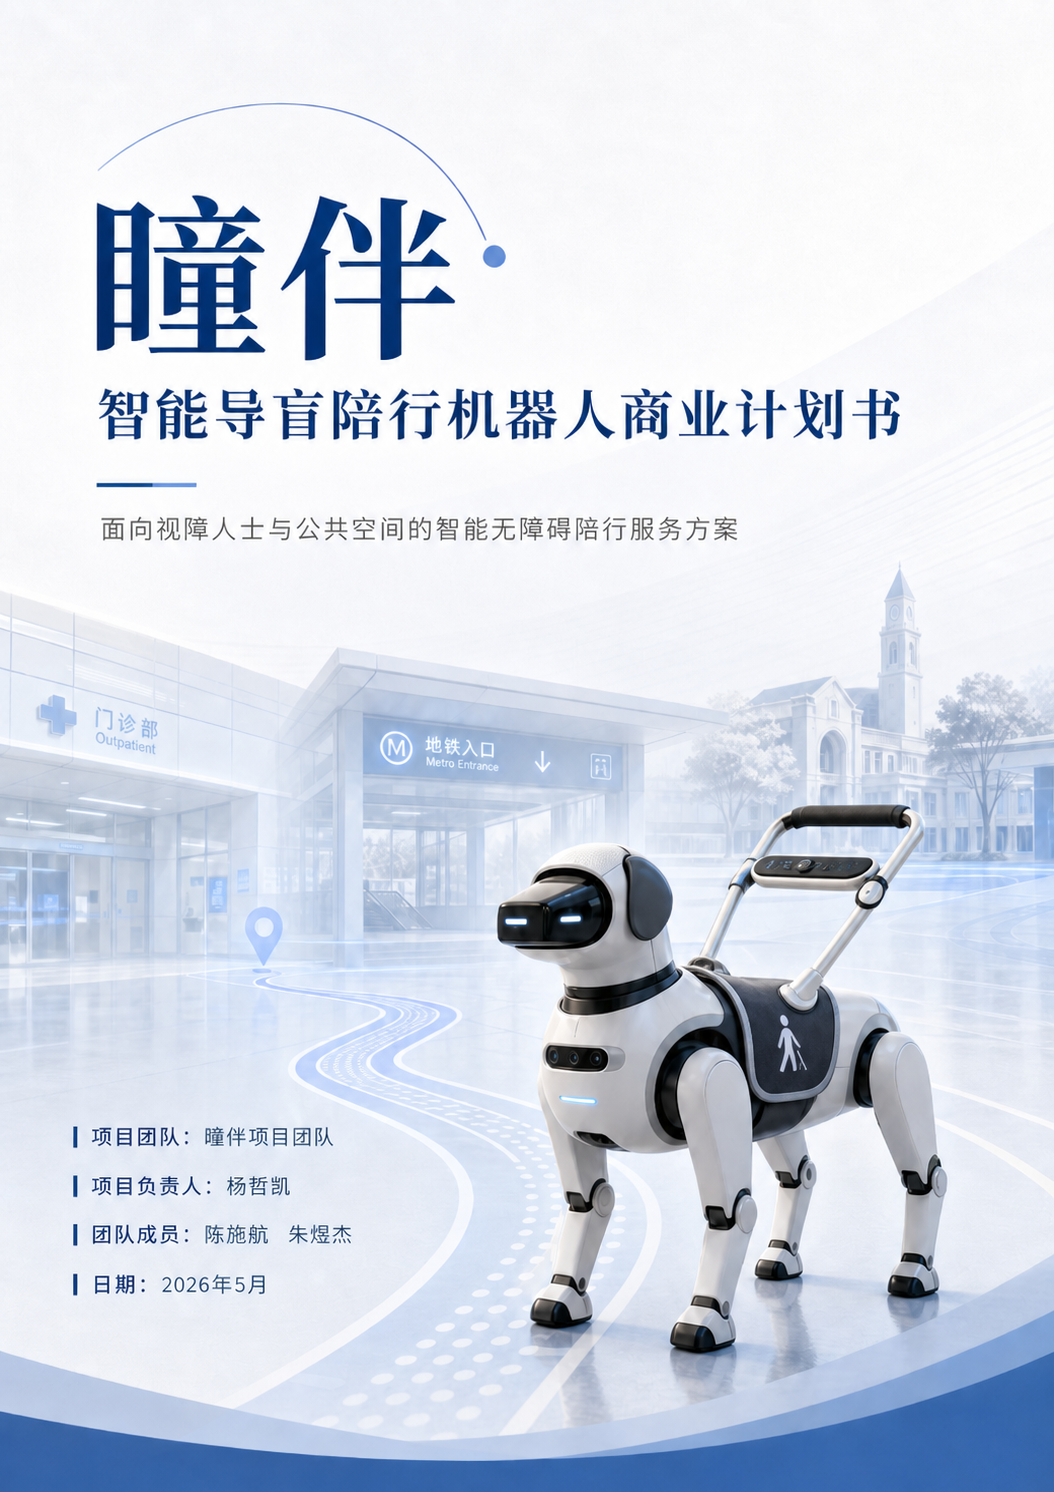
\includegraphics[width=\paperwidth,height=\paperheight]{FirstPage.png}%
  }%
}
\null
\clearpage

\pagenumbering{roman}
\tableofcontents
\clearpage
\pagenumbering{arabic}

"我们无法让世界少一分黑暗，但科技可以化作那束光。"—— 瞳伴，用智能导引技术帮助视障者更安全、更独立地出行。

\section{项目简介}

瞳伴是一款为视障人士、低视力老人和特殊出行人群打造的智能导盲犬形态陪行机器人，提供“硬件感知+室内外导航+场景地图+运营维护”的完整辅助出行服务。

我们的客户分为两类：一类是C端个人家庭用户，需要安全、可靠、降低家属陪护压力的出行工具；另一类是B端场景客户，包括医院、景区、交通枢纽和政务大厅等，需要借助智能无障碍设施提升公共服务体验。

项目的核心创新在于将真实导盲犬的陪伴感、盲杖的低门槛与机器人自动导航的确定性融合。传统工具难以判断复杂路口和室内目的地，而瞳伴通过激光雷达建图与柔性牵引手柄，让设备成为有温度的“向导”。这一创新直击视障人群“看不见路、找不到点、不敢独自进入陌生空间”的痛点，将公共空间静态的无障碍设施升级为动态的陪行服务。

项目所在的辅助出行与无障碍服务市场正迎来快速增长。需求端，全国视障人士超过1700万，65岁及以上人口已达22023万人（国家统计局《2024年统计公报》，占比15.6\%），而全国在役导盲犬不足200条——供给缺口高达数万倍。产业端，根据前瞻产业研究院数据，2024年中国康复辅具市场规模已突破800亿元，年均增长7\%--8\%；银发经济总规模约30万亿元，出行辅助与康养辅具占比2\%--5\%，对应6000亿--1.5万亿元市场空间。同时，中国服务机器人市场规模约500--800亿元，年增长率20\%--30\%（中国电子学会），其中公共服务机器人是增速最快的细分赛道。瞳伴所处的“智能辅具 + 公共服务机器人 + 银发出行”交叉赛道，具备千亿级的潜在市场空间。

我们依靠行业领先的技术体系与清晰的商业路径将上述优势落地。在技术端，凭借2D/3D激光雷达、深度摄像头与SLAM室内外建图算法，实现了复杂环境下的高精度多传感器融合感知与连续导航，并通过独创的柔性牵引控制保障人机共行安全。在落地端，采取“先B端标杆试点、后C端规模扩展”的路径，结合“设备租赁+场景建图+年度运维”的商业模式，建立长期竞争优势。

围绕这一目标，我们组建了一支分工明确的团队。团队由曾获全国大学生创业计划竞赛金奖的成员领衔，职能覆盖底盘硬件研发、SLAM导航算法、B端市场拓展与场景运营交付。项目还引入了由资深康复辅具专家、无障碍环境研究人员以及专业导盲犬训练机构导师组成的顾问团队进行背书。顶尖技术研发与权威行业顾问的组合，保障了技术路线的可行性，并确保产品契合国家无障碍服务标准与视障人士真实使用习惯。

在投资回报方面，本项目具备较强的盈利能力和增长潜力。基于稳健的财务测算，项目未来五年的营业收入将从初期的180万元攀升至2030年的6100万元，净利润将突破1680万元。投资人以300万元获取12\%股权，将在五年内分享科技与银发经济双重红利下的经营分红，并可在公司完成20个以上B端场景复制后，通过下一轮融资的估值跃升或产业并购，实现数倍的资本回报。

本项目本轮计划融资300万元，出让公司12\%股权，另有创始团队自筹的50万元启动资金。资金将专项用于核心业务，具体包括：工程样机迭代升级、激光雷达等核心传感器集中采购、室内无障碍导航地图平台开发，以及在2至3家三甲医院和头部景区完成标杆试点建设与安全测试认证。这笔投入将帮助瞳伴跨越验证期，迅速建立商业化规模复制的基础。

\section{产品与服务}

\subsection{应用背景}

\PlanItem{据中国残联统计，我国视障人士超过1700万，独立出行是他们面临的最大挑战之一。困难不只是“看不见路”，更在于无法稳定判断环境变化——道路上的共享单车、临时施工、低垂树枝、玻璃门、台阶边缘、闸机入口和密集人流，都可能带来安全隐患。在医院、景区、地铁站等室内或半室内空间中，传统导航难以准确提示楼层、诊室、卫生间、电梯和服务窗口的位置，导致用户即使抵达建筑入口，也难以顺利到达最终目的地。}

\PlanItem{现有辅助工具各有局限。普通盲杖价格低、携带方便，但感知范围有限，主要识别近处、低位障碍；电子盲杖可提供超声波提示，但多数仍停留在“发现障碍后报警”层面，无法主动完成目的地导引；真实导盲犬提供出色的陪伴与引导体验，但训练周期长、供给数量少、饲养成本高，且易受公共场所理解不足和管理规则差异的制约。}

\PlanItem{瞳伴的产品机会来自这三类工具之间的空白地带：它要像盲杖一样易于获取，像导盲犬一样提供方向感与陪伴感，同时又像智能机器人一样具备环境感知、路径规划和场景复制能力。因此，本项目将产品定位为"导盲犬形态的智能陪行机器人"，重点服务视障人士、低视力老人以及景区、医院、交通枢纽等公共空间的无障碍导引需求。}

\begin{figure}[H]
  \centering
  \includegraphics[width=0.85\textwidth]{p1.png}
  \caption{视障者在公共空间中面临的导引困境}
\end{figure}

\subsection{产品简介}

\PlanItem{瞳伴由导盲犬形态移动底盘、激光雷达感知系统、深度视觉系统、语音交互系统、牵引反馈手柄、边缘计算模块、电池管理模块和远程运维平台构成。产品采用低重心、小体积、低速平稳行进的设计，外观形态弱化机械设备的冰冷感，使用户在心理上更自然地将其视为"陪行伙伴"。}

\begin{figure}[H]
  \centering
  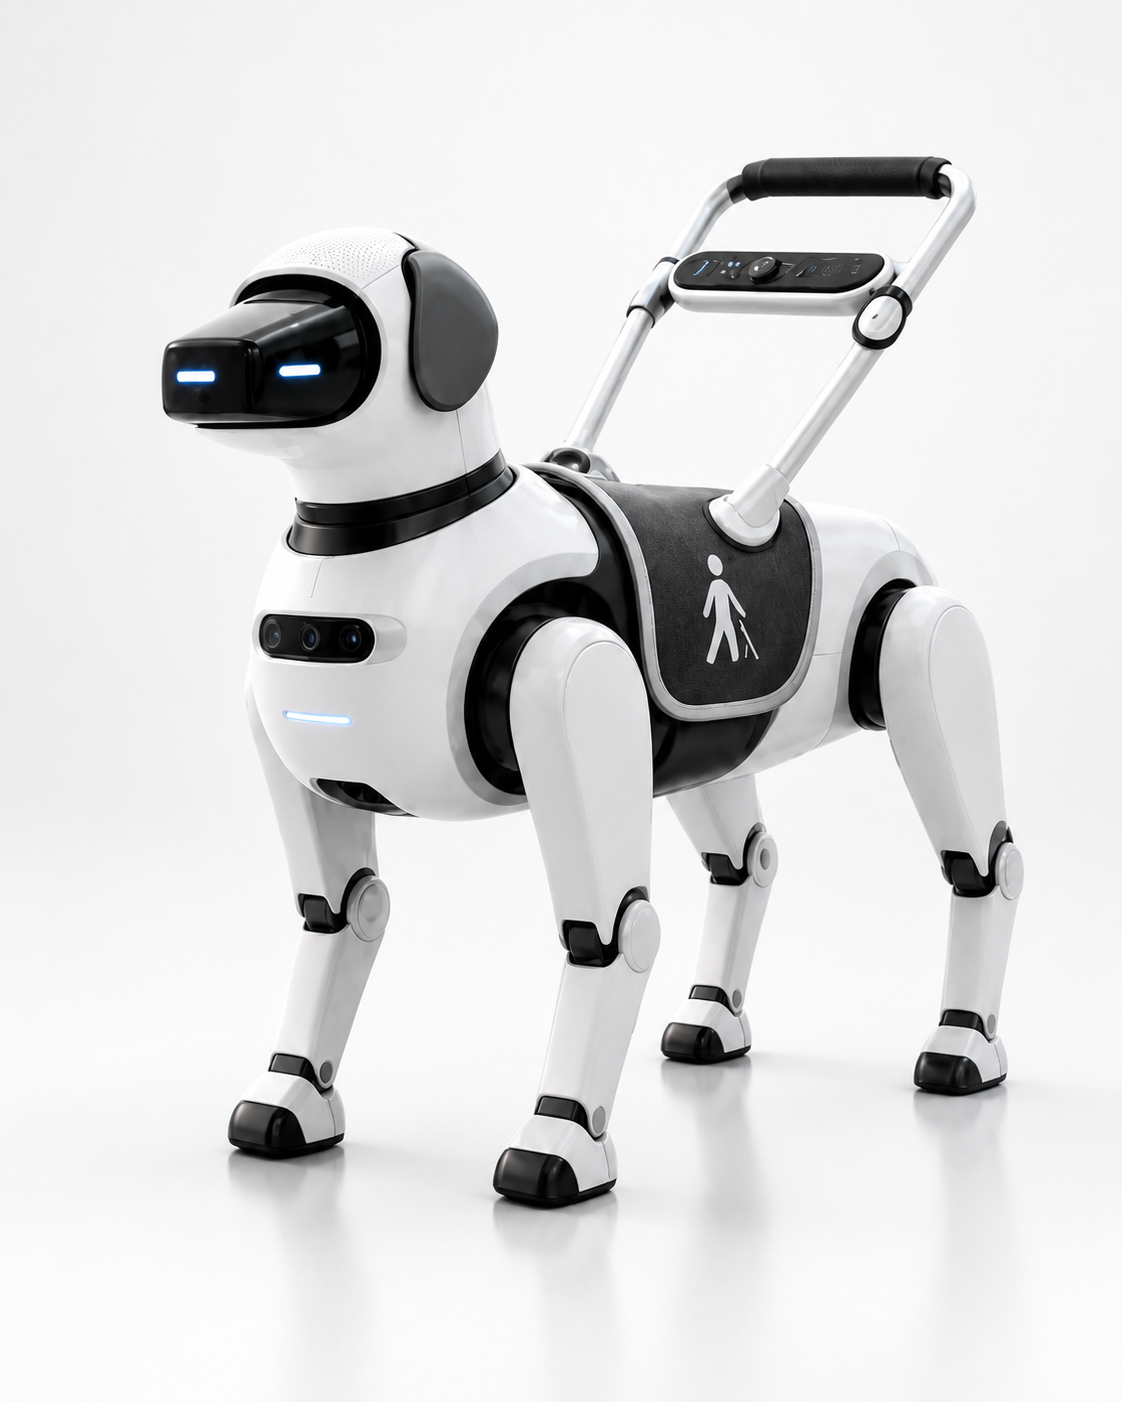
\includegraphics[width=0.85\textwidth]{p2.png}
  \caption{瞳伴产品概念渲染图}
\end{figure}

\PlanItem{产品使用时，用户通过语音或预设按钮输入目的地，例如“带我去三号诊室”“去景区出口”“找最近的卫生间”。设备接收指令后，结合已有地图和实时环境感知进行路径规划，通过牵引手柄传递前进、转向、减速和停止等方向信息，并辅以语音播报关键节点。用户既无需持续查看手机屏幕，也不必记住复杂路线，只需跟随手柄方向和语音提示即可完成移动。}

\PlanItem{瞳伴定位为一种可量产、可租赁、可部署、可持续运维的智能辅助产品。对于个人用户，它是日常出行和陌生场景中的安全辅助工具；对于景区、医院、车站等公共空间，它是提升无障碍服务能力的智能设施；对于残联、社区和公益机构，它是可集中采购、共享使用、降低服务成本的新型辅助器具。}

\begin{figure}[htbp]
  \centering
  \begin{tikzpicture}[
    node distance=1.1cm,
    module/.style={draw, rounded corners, minimum width=3cm, minimum height=0.9cm, align=center},
    core/.style={draw, rounded corners, minimum width=3.6cm, minimum height=1cm, align=center, fill=gray!12},
    arrow/.style={-{Stealth[length=2.2mm]}, thick}
  ]
    \node[core] (robot) {导盲犬形态\\智能陪行机器人};
    \node[module, above left=of robot] (lidar) {激光雷达\\深度视觉};
    \node[module, above right=of robot] (compute) {边缘计算\\路径规划};
    \node[module, below left=of robot] (handle) {牵引手柄\\震动反馈};
    \node[module, below right=of robot] (voice) {语音交互\\紧急求助};
    \node[module, below=1.45cm of robot] (cloud) {地图平台\\远程运维};
    \draw[arrow] (lidar) -- (robot);
    \draw[arrow] (compute) -- (robot);
    \draw[arrow] (robot) -- (handle);
    \draw[arrow] (robot) -- (voice);
    \draw[arrow] (robot) -- (cloud);
  \end{tikzpicture}
  \caption{产品总体构成示意图}
\end{figure}

\subsection{产品功能}

\PlanItem{室外避障通行是瞳伴的基础能力。产品通过激光雷达、深度摄像头和超声波传感器识别行人、墙体、车辆边缘、路障、台阶、低矮障碍物和临时施工区域，在用户步行速度范围内实时调整行进路线。相比普通盲杖只能探知1米内的低位障碍，瞳伴可提前发现20米以外的风险，并通过牵引反馈和语音提示同时提醒用户。}

\begin{figure}[H]
  \centering
  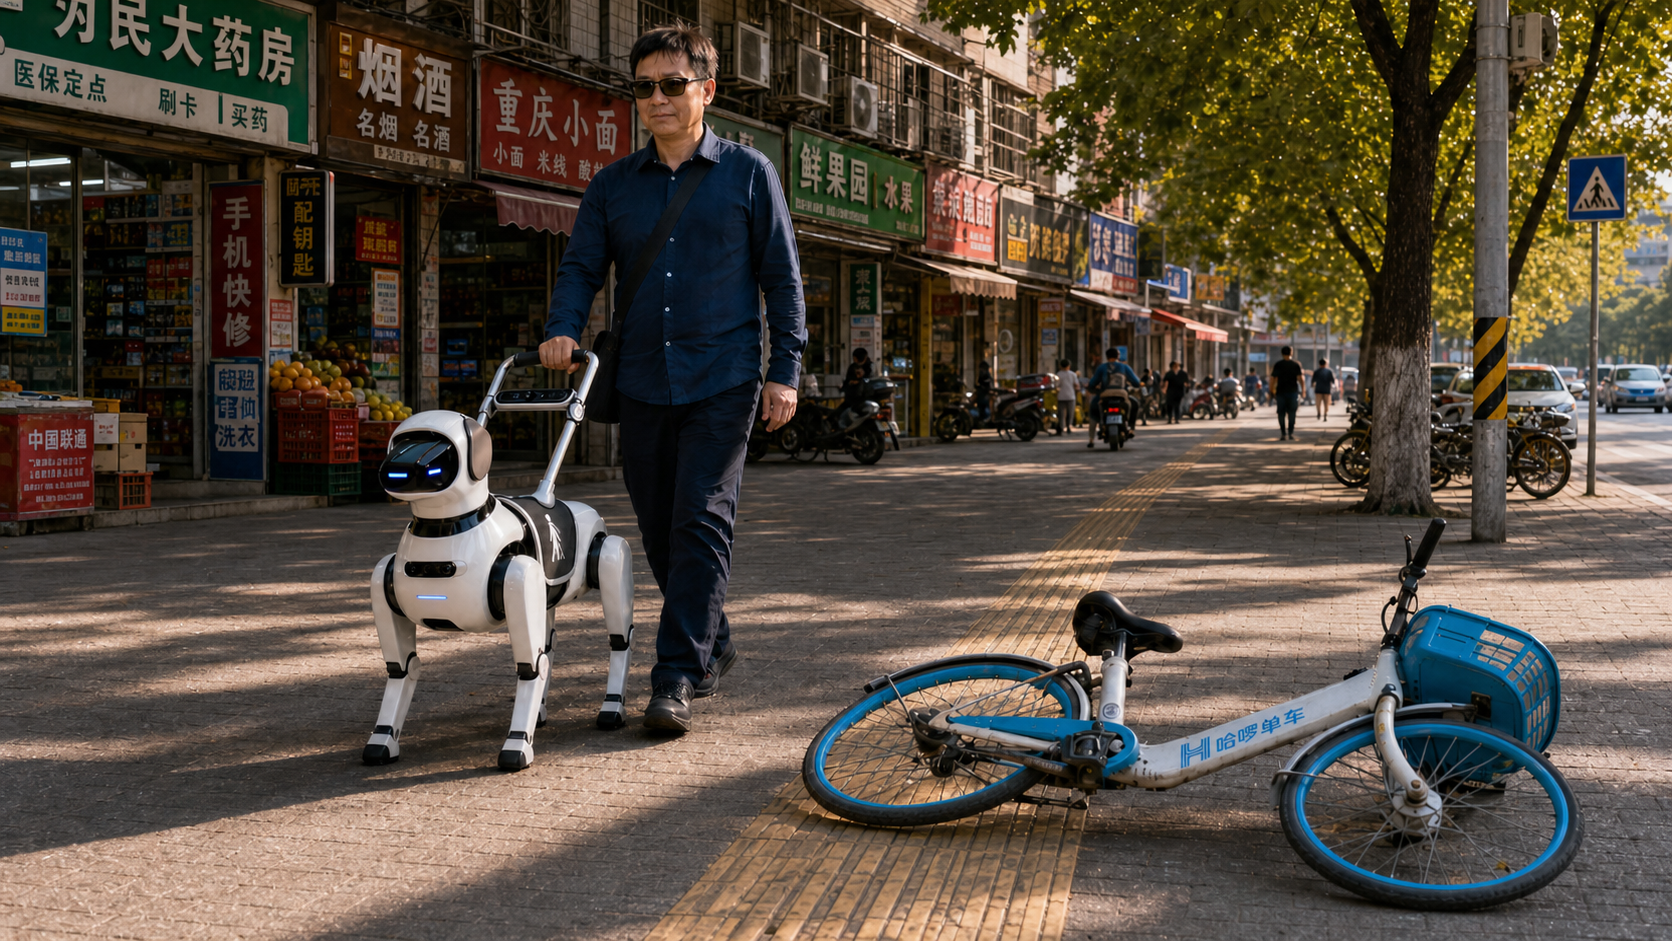
\includegraphics[width=0.85\textwidth]{p3.png}
  \caption{瞳伴室外避障使用场景}
\end{figure}

\PlanItem{室内精准导引是瞳伴区别于所有现有方案的核心突破。GPS在建筑内部完全失效，而对视障人士来说，找不到诊室、卫生间、电梯入口才是最大的困扰。项目为景区、医院、博物馆、政务大厅和交通枢纽等场景建立室内地图和语义点位库，将入口、服务台、电梯、卫生间、诊室、展厅、售票处、出口等位置逐一标注。用户说出目的地，设备即可在室内空间完成路径规划并引导到达。}

\begin{figure}[H]
  \centering
  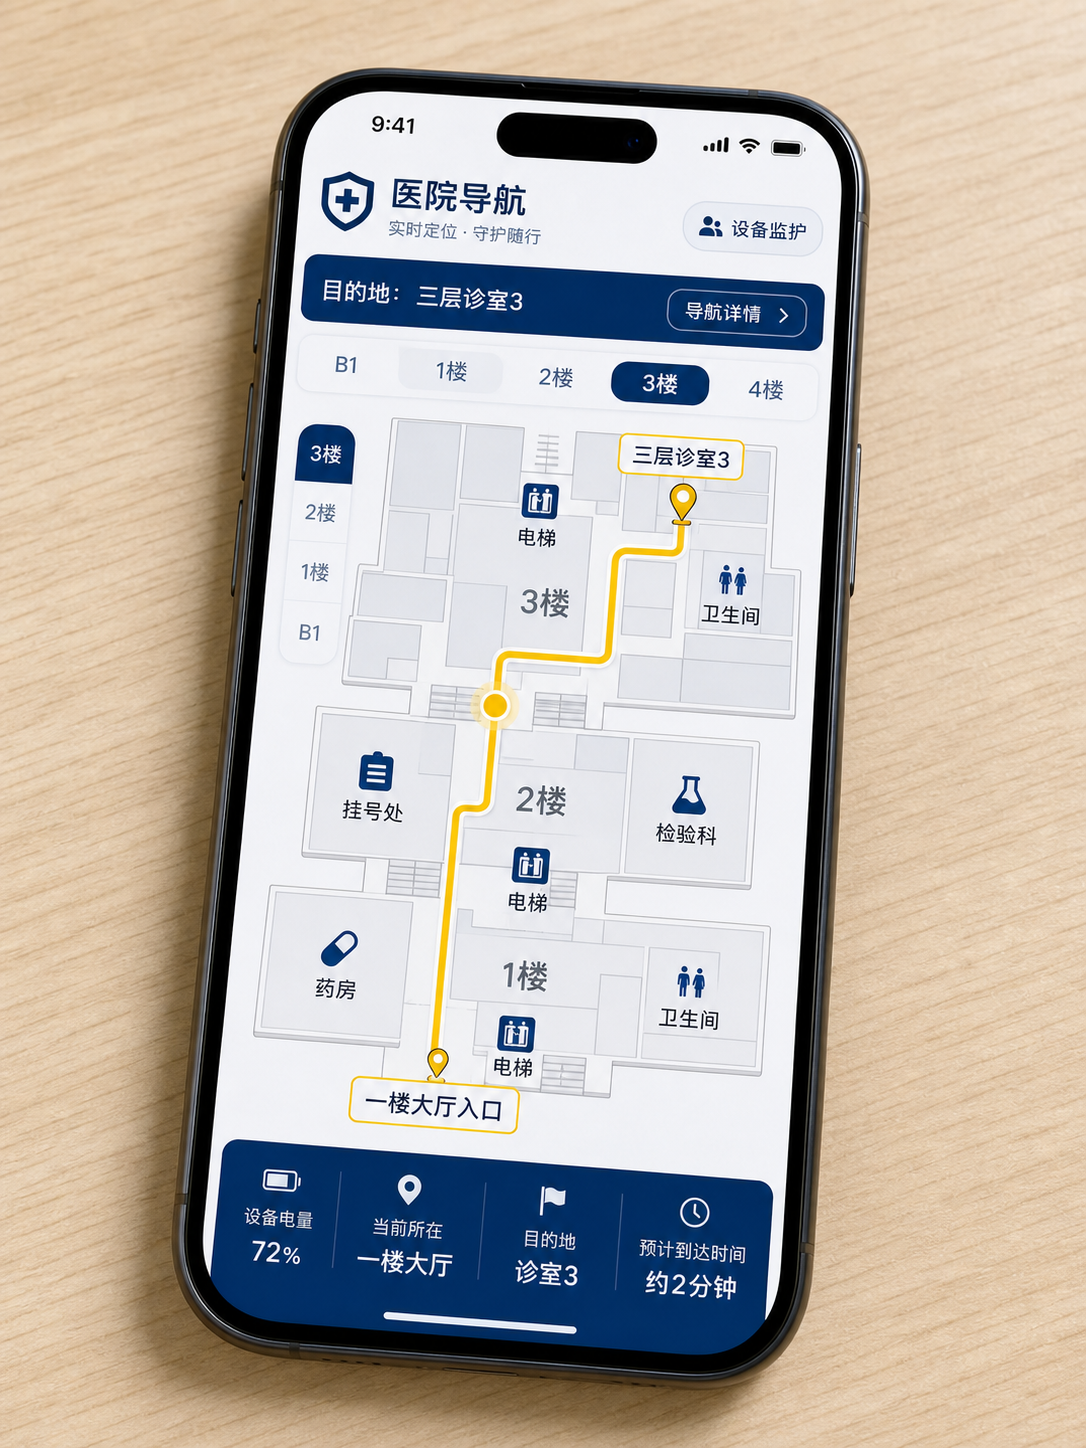
\includegraphics[width=0.6\textwidth]{p4.png}
  \caption{配套手机APP——家属或工作人员可实时查看设备位置与导航路线}
\end{figure}

\PlanItem{景区无障碍游览是项目早期重点切入的场景之一。视障游客不应只是"被带进去"再"带出来"——瞳伴可以为视障游客提供无障碍路线推荐、景点讲解播报、休息点提示、卫生间导引和返回入口服务，让他们真正参与到游览体验中。}

\PlanItem{医院与公共服务导引是另一高频刚需场景。医院内部科室复杂、楼层多、排队点位密集，给视障人士和低视力老人带来极大不便。瞳伴可根据医院导诊地图引导用户到达挂号处、诊室、检查室、取药窗口和出口，既减少了人工导诊压力，也提升了特殊群体的就医体验。}

\PlanItem{安全守护贯穿所有功能。设备提供一键求助、实时位置共享、低电量提醒、异常停留告警和远程运维监控。当检测到定位异常、障碍物过近、用户突然停顿或电量不足时，设备自动减速或停止，并通过语音和后台同时通知相关人员。手柄上保留了物理急停键，任何时候用户都可以一键让设备停下。}

\begin{table}[H]
  \centering
  \caption{产品核心功能}
  \begin{tabularx}{\textwidth}{>{\raggedright\arraybackslash}p{3cm} >{\raggedright\arraybackslash}X}
    \toprule
    功能模块 & 具体说明 \\
    \midrule
    激光雷达避障 & 识别墙面、行人、立柱、台阶边缘和临时障碍，实时调整行进路线 \\
    室内导引 & 基于预构建地图和语义点位库，实现入口、诊室、展厅、卫生间等点位导航 \\
    景区导览 & 在景区内提供无障碍路线、讲解播报、休息点推荐和返回入口服务 \\
    牵引反馈 & 通过手柄方向力和震动提示传递前进、转向、减速和停止信号 \\
    安全守护 & 提供一键求助、实时位置共享、低电量提醒和异常滞留告警 \\
    \bottomrule
  \end{tabularx}
\end{table}

\subsection{核心技术}

\PlanItem{多传感器融合感知是瞳伴的感知底座。激光雷达负责高精度测距与环境轮廓识别（探测距离≥20米，测距精度±3cm，角度分辨率≤1°），深度摄像头负责识别斑马线、门牌、电梯、闸机、扶梯、台阶等语义信息（有效识别距离0.5--10米），超声波传感器负责补充1--3米近距离盲区，惯性测量单元负责姿态估计与运动状态判断。四种传感器各有盲区，但叠加在一起，才能在复杂光照、密集人流和室内空间中保持可靠。}

\PlanItem{室内外连续导航让瞳伴区别于任何只靠GPS的方案。室外场景结合北斗/GPS、视觉识别和局部避障完成通行；一进入建筑内部，立刻切换为激光SLAM建图（定位精度2--5cm）、蓝牙信标、二维码点位和语义地图的综合定位。关键不是设备能不能移动，而是它在公共空间中是否始终知道自己在哪、用户要去哪、路线上有哪些风险——路径规划成功率目标≥95\%。}

\PlanItem{人机共行控制是视障陪行场景独有的技术挑战。普通配送机器人只需要计算自己怎么从A到B，但瞳伴牵引的是一个人。使用者的步幅、心理安全感、握持习惯、转弯半径和突发停顿,每一个变量都影响安全。瞳伴将陪行速度严格控制在0.5--1.0 m/s（正常步行速度范围内），急停响应时间＜100ms，单次充电续航目标≥6小时。设备通过柔性牵引、偏航提醒和主动让行，成为一个"引导者"而不是拖拽人的机器。}

\PlanItem{场景地图运维决定了产品能否从一台样机变成一个可复制的业务。产品进入景区、医院、地铁站等场景前，需要完成地图采集、点位标注、无障碍路线审核和危险区域标记；投入使用后，施工改道、展厅调整、科室搬迁、人流变化——地图必须持续更新。有了地图运维能力，每进入一个新场景就不再是从零开始，而是在标准化流程上做适配。}

\begin{figure}[H]
  \centering
  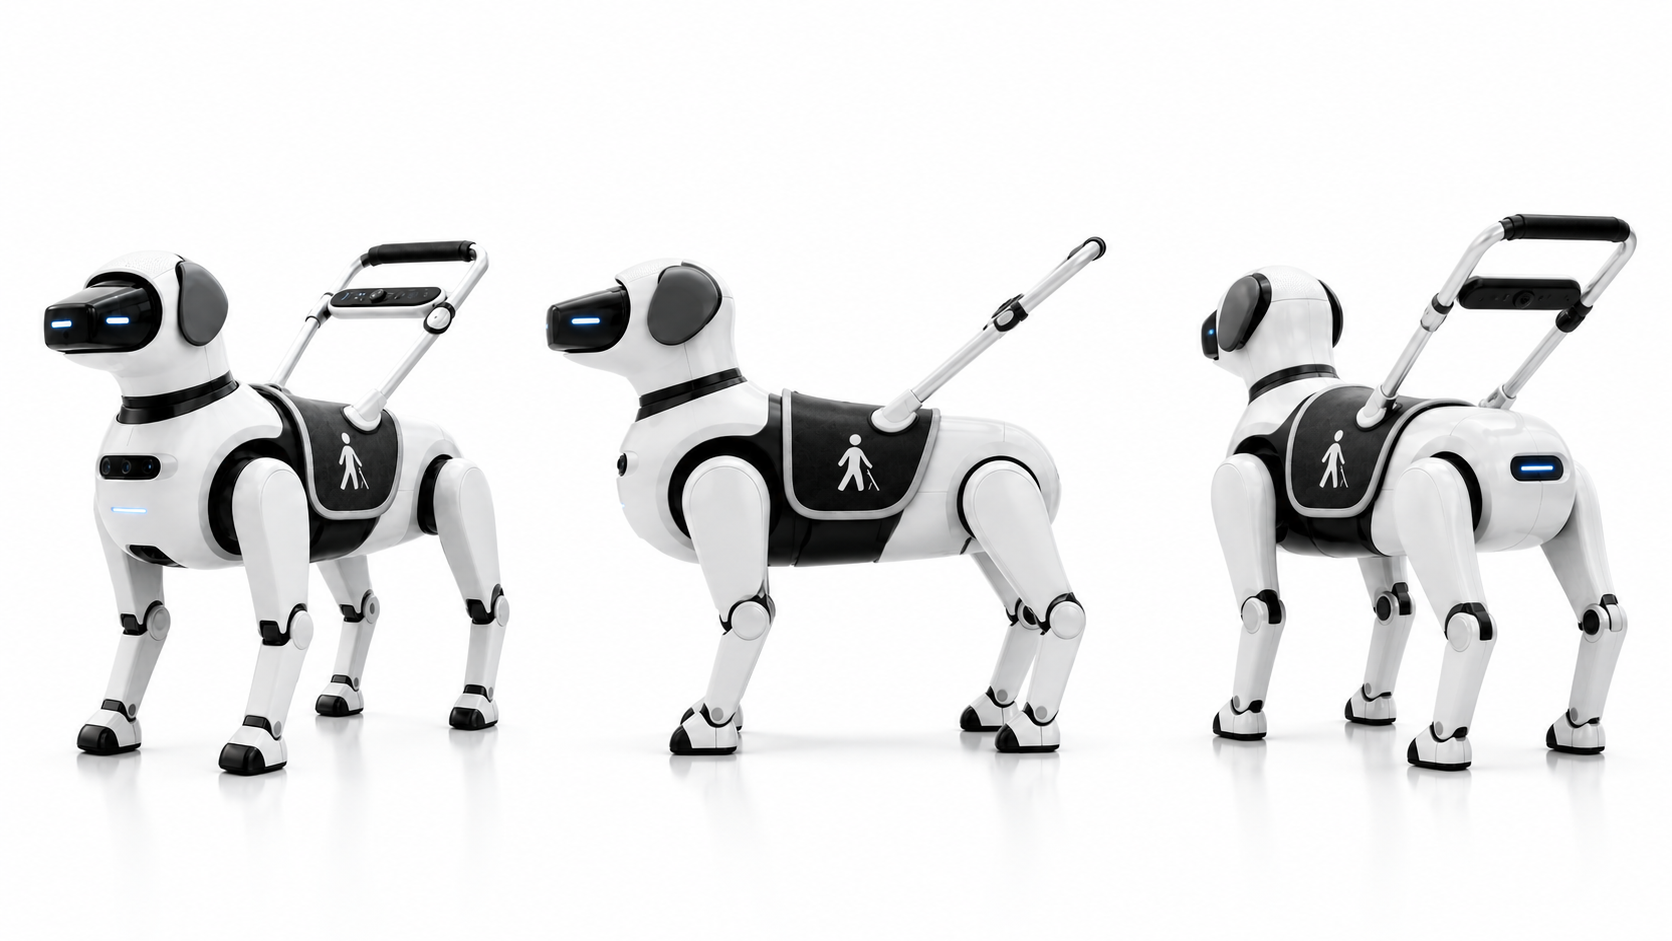
\includegraphics[width=0.85\textwidth]{p5.png}
  \caption{瞳伴产品多角度展示}
\end{figure}

\begin{figure}[htbp]
  \centering
  \resizebox{0.9\textwidth}{!}{%
  \begin{tikzpicture}[
    node distance=0.9cm,
    flowstep/.style={draw, rounded corners, minimum width=2.5cm, minimum height=0.85cm, align=center},
    arrow/.style={-{Stealth[length=2mm]}, thick}
  ]
    \node[flowstep] (sense) {多传感器\\环境感知};
    \node[flowstep, right=of sense] (map) {SLAM 建图\\室内定位};
    \node[flowstep, right=of map] (plan) {路径规划\\风险判断};
    \node[flowstep, right=of plan] (interact) {语音提示\\牵引反馈};
    \node[flowstep, right=of interact] (safe) {异常停车\\后台告警};
    \draw[arrow] (sense) -- (map);
    \draw[arrow] (map) -- (plan);
    \draw[arrow] (plan) -- (interact);
    \draw[arrow] (interact) -- (safe);
  \end{tikzpicture}
  }
  \caption{核心技术路线示意图}
\end{figure}

\subsection{服务体系}

\PlanItem{面向 B 端场景客户，瞳伴提供“设备投放 + 场景建图 + 用户培训 + 运维巡检 + 后台管理”的一体化服务。项目团队先对场景进行路线勘察和地图采集，再部署设备并培训现场工作人员，后续通过远程后台查看设备状态、路线成功率、故障记录和用户反馈。}

\PlanItem{面向 C 端个人客户，项目提供购买、长租、短租和共享使用等不同服务方式。高频出行用户可以购买个人版设备，普通家庭可以选择月租或季租，景区和医院中的临时用户则可以现场预约使用。这一设计有效降低了首次使用门槛，使用户先在公共场景中建立信任，再逐步导入个人端市场。}

\PlanItem{售后服务包括设备维修、软件更新、地图更新、用户训练和安全回访。由于本产品直接关系到出行安全，售后不只是普通维修，而是产品体验的一部分。项目将建立设备档案和使用记录，对故障高发点、路线失败点和用户不适应环节进行持续优化。}

\subsection{产品优势与先进性}

\PlanItem{与普通盲杖（市价30--500元）相比，瞳伴的优势在于感知距离从1米延伸至20米以上，识别对象更丰富，且可主动规划路线；与超声波电子盲杖（市价300--3,000元）相比，项目不只是提示障碍，更提供完整的室内导引服务；与真实导盲犬（单只训练成本19.6万元，全国在役不足200条，年产出仅35--40条，覆盖视障人群不足0.003\%）相比，项目具备可量产、可租赁、可集中投放、可远程运维的优势；与国际竞品Glidance Glide（定价\$1,499+\$30/月订阅，2026年首发仅限北美和英国）相比，瞳伴更贴合中国公共空间场景并具备本地化场景运维能力；与手机导航相比，项目更适合不便看屏幕、不熟悉路线或身处复杂室内空间的用户。}

\PlanItem{项目的先进性还体现在公共空间服务化上。许多无障碍设施是静态的，例如坡道、电梯和盲道，但视障人士真正进入空间后，仍需要知道“下一步往哪里走”。瞳伴将无障碍服务从静态设施延伸至动态陪行，将单个用户工具升级为场景级服务系统。}

\PlanItem{产品采用导盲犬形态，旨在使用户更自然地理解设备行为。牵引式交互比单纯语音播报更直观，低速陪行比完全自主高速移动更安全，柔和外观比冰冷机器更易被公共空间接受。这种产品形态在设计上兼顾了技术功能、用户心理与场景接受度。}

\subsection{未来研发规划}

\PlanItem{研发将分三个阶段推进。早期聚焦工程样机稳定性——完成底盘可靠性、激光雷达避障、牵引手柄反馈、室内地图导航和基础语音交互，保证设备能在校园、展馆等半封闭场景中安全运行。中期转向场景适配——面向景区、医院和交通枢纽分别建立标准地图模板、点位标注规范和路线审核流程，重点攻克人流密集、路线交叉、楼层变化和临时施工等复杂情况。后期发力智能服务升级——随着使用数据积累，开发个性化路线偏好、用户步速适配、多人预约调度、设备自动回桩充电和多设备协同管理，从单台陪行设备发展为公共空间无障碍智能服务平台。}

\section{行业与市场}

\subsection{行业特征}

\PlanItem{政策层面，《中华人民共和国无障碍环境建设法》正式施行后，公共场所、交通设施、信息服务和社会服务等领域的无障碍建设要求从"倡导"变成了"义务"。景区、医院、政务大厅、交通枢纽等空间需要建设的不仅是坡道和电梯，还有精细化的导引、信息提示和陪行服务。瞳伴所在的无障碍环境建设、残疾人辅助器具、智慧公共服务和银发经济交叉区域，正在获得持续的政策推动。}

\PlanItem{经济层面，视障辅助器具与服务过去主要依赖公益捐赠和政府采购，付费意愿不强。但情况正在变化——公共服务数字化、智慧景区建设和康养消费升级，让场景方开始算一笔清晰的账：医院希望减少人工导诊压力，景区希望提升服务评价和品牌形象，交通枢纽希望降低特殊旅客人工陪同成本，残联和社区希望用有限预算服务更多人群。这些需求过去没有好的产品来承接，现在有了。}

\PlanItem{社会层面，老龄化叠加特殊群体公共参与意识觉醒，需求不再是小众话题。低视力老人、视障人士、行动不便人群以及短期眼部疾病患者，都可能在陌生公共空间中遭遇导航困难——这已经不只是"帮助少数人"的问题，而是城市文明、公共服务公平和社会包容度的直接体现。}

\PlanItem{技术层面，激光雷达、SLAM建图、低速移动机器人、语音交互和边缘计算已经过了概念验证期。配送机器人、清洁机器人和导览机器人在商场、园区和酒店的落地，证明了低速移动设备在公共空间中的可行性。将这些技术迁移至视障陪行，路径上不存在原理性障碍，挑战在于安全冗余、人机牵引和无障碍交互的针对性适配。}

\subsection{市场需求}

\PlanItem{需求端由三类人群共同构成。第一类是长期视障人士，他们需要更稳定、更安全、更能进入陌生空间的独立出行工具；第二类是低视力老人，他们可能缺乏熟练使用盲杖和智能手机导航的能力，却存在就医、办事、游览和社区活动等现实需求；第三类是公共场景中的临时需求人群，包括短期眼部疾病患者、夜间低视力游客和行动不便者。}

\PlanItem{个人端需求的核心不是购买一台高科技设备，而是获得更高的出行确定性。视障人士出门前最担心的是路线是否变化、是否有人流冲突、是否能找到具体入口和目的地。瞳伴提供的价值，是将“需要别人带路”这一不确定过程，转化为“设备可陪行、路线可规划、异常可求助”的服务保障过程。}

\PlanItem{B 端场景需求同样明确。景区需要提供无障碍游览和讲解服务，医院需要把患者从入口带到具体诊室、检查室和取药窗口，交通枢纽需要在安检、候车、换乘和出站之间提供连续导引，政务大厅需要帮助特殊人群完成办事流程。与单纯面向个人销售相比，先进入 B 端场景更容易形成展示案例、稳定回款和规模复制。}

\begin{table}[H]
  \centering
  \caption{目标市场细分}
  \begin{tabularx}{\textwidth}{>{\raggedright\arraybackslash}p{3cm} >{\raggedright\arraybackslash}p{4cm} >{\raggedright\arraybackslash}X}
    \toprule
    市场类型 & 主要客户 & 核心需求 \\
    \midrule
    公共服务市场 & 残联、社区、政务大厅 & 提供辅助器具服务，提升公共服务公平性 \\
    医疗导引市场 & 医院、康复中心、体检中心 & 降低导诊压力，帮助患者到达诊室和检查点 \\
    文旅无障碍市场 & 景区、博物馆、展馆 & 提供无障碍游览、智能讲解和服务品牌升级 \\
    个人出行市场 & 视障人士、低视力老人及家庭 & 提升独立出行能力，降低家属陪同压力 \\
    \bottomrule
  \end{tabularx}
\end{table}

\subsection{市场调研}

\PlanItem{为使项目方案更贴近真实需求，本计划书设置了调研框架，主要面向三类对象：视障人士及低视力老人、景区/医院等公共空间管理者、残联和社区服务人员。调研重点不只是“是否需要导盲设备”，而是围绕出行场景、付费意愿、信任顾虑、服务流程和安全责任展开。}

\PlanItem{从调研结果看，不同对象的关注点差异明显。视障人士和低视力老人最在意安全性、路线准确性、操作简单程度和突发情况求助能力——相比炫酷外形，用户更关心设备能否稳定停下、能否清楚提示方向、能否在复杂室内找到具体点位、会不会因为设备故障而陷入更危险的处境。}

\PlanItem{景区和医院的关注点则各有侧重。景区更重视无障碍服务形象、游客体验、讲解功能和设备展示效果；医院更重视路线准确、导诊效率、排队点位和工作人员协同；交通枢纽则更重视安全责任、换乘路线和异常情况处置。不同场景都认可智能导引的价值，但也都要求产品必须配备清晰的运维机制。}

\PlanItem{残联和社区则更关注设备共享、培训成本、公益采购和低收入人群可及性。一次性高价采购对这类客户压力较大，租赁、联合采购、公益赞助和共享服务点更容易被接受。}

\begin{table}[H]
  \centering
  \caption{市场调研结论摘要}
  \begin{tabularx}{\textwidth}{>{\raggedright\arraybackslash}p{3cm} >{\raggedright\arraybackslash}X}
    \toprule
    调研对象 & 主要结论 \\
    \midrule
    视障人士及低视力老人 & 重视安全、简单、准确和求助功能，对价格较敏感，需要先体验再信任 \\
    景区/博物馆 & 关注无障碍服务形象、游览路线、讲解播报和游客评价提升 \\
    医院/公共服务机构 & 关注导诊效率、路线准确、工作人员配合和异常情况处理 \\
    残联/社区 & 关注共享使用、公益采购、培训成本和辅助器具可及性 \\
    \bottomrule
  \end{tabularx}
\end{table}

\subsection{市场定位}

\PlanItem{瞳伴的市场定位是“面向公共空间和个人出行的智能无障碍陪行服务商”。它不是普通消费电子或机器人玩具，而是服务视障人士、低视力老人和公共空间管理方的辅助器具与场景服务结合体。}

\PlanItem{项目早期定位以 B 端场景为主、C 端用户为辅。B 端选择景区、医院、校园、博物馆和残联服务中心等相对可控空间作为试点，原因是这些场景目的地明确、路线可建图、服务需求真实、管理方有社会责任和品牌展示需求。C 端则借助这些公共场景完成体验教育，让用户先行建立信任，再逐步导入家庭长租和个人购买市场。}

\PlanItem{从价格定位看，项目不走极低价路线，也非高端小众产品。合理定位应是“个人购买有门槛、场景共享可承受、公益采购可覆盖”。通过设备租赁、共享使用和政府/公益采购，降低单个用户承担的成本，让产品更适合大规模推广。}

\subsection{竞争分析}

\PlanItem{当前市场上的主要替代方案呈现明显的价格与能力断层。}

\PlanItem{普通盲杖价格30--500元，成本最低，但只能探知1米内的低位障碍，无路线规划，无室内定位。}

\PlanItem{超声波电子盲杖价格300--3,000元，增加了震动和蜂鸣提示，探测距离扩展到1--3米，但多数仍停留在"发现障碍后报警"层面，无法主动完成目的地导引。}

\PlanItem{真实导盲犬单只训练成本高达19.6万元（中国导盲犬大连培训基地，2021年），全国在役不足200条，年产出仅35--40条，对1700万视障人士覆盖率不足0.003\%。体验虽好，供给近乎为零。}

\PlanItem{手机导航免费，但对全盲或低视力用户操作困难，且GPS在室内完全失效，对复杂室内点位帮助极为有限。}

\PlanItem{国际导盲机器人Glidance Glide定价\$1,499加\$30/月订阅，预计2026年首发但仅限北美和英国，中国市场短期内无法触达。}

\PlanItem{人工陪同最为可靠，但成本高达200--500元/天，隐私感差，且不可能全天候覆盖。}

\PlanItem{这些替代方案共同的问题是：要么能力单一，要么供给稀缺，要么价格不可承受——这正是瞳伴的市场切入空间。}

\PlanItem{\textbf{在竞争策略上，本项目明确采取“错位竞争”策略。}我们不与百度地图、高德地图等互联网巨头在室外大范围通用导航上正面竞争，也不与大疆等纯硬件厂商拼激光雷达的硬件规模效应。瞳伴的差异化优势在于“可移动、可导引、可部署、可运营”，我们避开巨头资源高度集中的室外自动驾驶红海，专注景区、医院、地铁站等“最后一公里”室内微观导航与无障碍陪行服务，通过建立场景运维优势来实现差异化领先。}

\PlanItem{从竞争壁垒看，单一硬件并不构成长期壁垒，真正的壁垒来自场景数据、地图运维、用户信任和渠道资源的积累。谁能更早进入真实公共空间，积累无障碍路线数据、用户反馈、设备运行记录和场景交付经验，谁就更易于形成后续的复制优势。}

\begin{table}[H]
  \centering
  \caption{项目与主要替代方案对比}
  \begin{tabularx}{\textwidth}{>{\raggedright\arraybackslash}p{2.4cm} >{\centering\arraybackslash}p{2cm} *{3}{>{\centering\arraybackslash}X} >{\centering\arraybackslash}p{2cm}}
    \toprule
    方案类型 & 参考价格 & 避障能力 & 室内导引 & 陪伴体验 & 可规模部署 \\
    \midrule
    普通盲杖 & 30--500元 & 低（约1米） & 无 & 低 & 高 \\
    电子盲杖 & 300--3,000元 & 中（1--3米） & 无 & 低 & 中 \\
    真实导盲犬 & 训练成本19.6万元/只 & 高 & 中 & 高 & 极低（年35--40条） \\
    手机导航 & 免费 & 低 & 中（室外） & 低 & 高 \\
    人工陪同 & 200--500元/天 & 高 & 高 & 高 & 低 \\
    瞳伴 & 售价1.8--2.6万元/租赁1,200--2,000元/月 & 高（≥20米） & 高（2--5cm定位） & 中高 & 高 \\
    \bottomrule
  \end{tabularx}
\end{table}

\subsection{波特五力分析}

\PlanItem{产业内部竞争方面，目前市场上已存在普通盲杖、电子盲杖、手机导航、室内导览机器人和人工陪同服务，但真正针对视障人士公共空间陪行、同时具备激光雷达避障、室内地图和场景运维的产品仍属少数。现阶段直接竞争强度中等，未来随着机器人企业的进入，该赛道竞争可能增强。}

\PlanItem{潜在进入者威胁方面，机器人企业、互联网地图企业、智慧景区服务商和康养平台都有可能进入该领域。它们在技术、资金或渠道上具有一定优势，但视障陪行场景需要长期用户信任积累、无障碍服务理解和公共空间交付经验，因此新进入者仍需跨越场景验证这一门槛。}

\PlanItem{供方议价能力方面，项目关键零部件包括激光雷达、深度摄像头、边缘计算模块、电池、电机和控制板。部分核心传感器短期内价格偏高，供应商议价能力中等偏强。项目应通过标准化选型、建立备选供应商和逐步扩大采购量来降低供应链风险。}

\PlanItem{买方议价能力方面，B 端客户包括景区、医院、残联和公共服务机构，采购流程较为审慎，往往会综合比较价格、服务效果和安全责任，议价能力较强。项目应通过租赁模式、示范案例、运维服务和社会价值证明降低客户决策难度。}

\PlanItem{替代品威胁方面，普通盲杖、电子盲杖、导盲犬、人工陪同和手机导航都能满足部分需求，但它们分别存在感知范围有限、供给不足、人力成本高或室内定位不足等问题。瞳伴的关键在于通过“设备 + 地图 + 运维”提供更完整的场景化解决方案，以此有效降低替代品的威胁。}

\begin{table}[H]
  \centering
  \caption{波特五力分析摘要}
  \begin{tabularx}{\textwidth}{>{\raggedright\arraybackslash}p{3.2cm} >{\centering\arraybackslash}p{2.2cm} >{\raggedright\arraybackslash}X}
    \toprule
    分析维度 & 强度判断 & 说明 \\
    \midrule
    产业内部竞争 & 中 & 现有替代方案较多，但场景化智能陪行产品仍少 \\
    潜在进入者威胁 & 中高 & 机器人、地图、文旅服务企业可能进入 \\
    供方议价能力 & 中高 & 激光雷达、边缘计算等核心部件短期成本较高 \\
    买方议价能力 & 高 & B 端客户采购谨慎，重视安全和成本 \\
    替代品威胁 & 中 & 盲杖、导盲犬和人工陪同可替代部分功能 \\
    \bottomrule
  \end{tabularx}
\end{table}

\subsection{SWOT 分析}

\PlanItem{优势方面，项目具有明确的社会价值和场景价值，能够同时满足视障人士独立出行、公共空间无障碍升级和景区/医院服务提质需求。产品融合了激光雷达、室内地图、牵引反馈和语音交互，差异化程度高，且适合通过 B 端场景实现批量投放。}

\PlanItem{劣势方面，项目早期研发难度和安全责任较高，对场景地图、设备稳定性、用户训练和售后运维要求都比较严格。相比普通盲杖，产品价格更高；相比成熟机器人品类，视障陪行场景对安全与信任的要求更为严苛，市场教育周期也更长。}

\PlanItem{机会方面，无障碍环境建设、银发经济、智慧文旅和公共服务数字化都在持续推进。景区、医院、交通枢纽和政务大厅对无障碍服务有真实改进需求，而目前市场上可同时提供智能导引、场景地图和陪行服务的成熟产品依然较少。}

\PlanItem{威胁方面，未来可能出现机器人企业、互联网地图企业、智能硬件企业进入该赛道，带来技术和资金竞争；同时，若早期试点中出现安全事故或用户体验不佳，将严重影响项目声誉。因此，项目必须坚持小范围验证、低速运行、人工兜底和稳步复制的原则。}

\begin{table}[H]
  \centering
  \caption{瞳伴 SWOT 分析}
  \begin{tabularx}{\textwidth}{>{\raggedright\arraybackslash}p{2.6cm} >{\raggedright\arraybackslash}X}
    \toprule
    类型 & 主要内容 \\
    \midrule
    优势 & 技术组合差异化明显，社会价值强，适合 B 端场景批量投放，可形成地图与运维服务收入 \\
    劣势 & 早期研发和安全验证成本高，用户信任建立慢，个人端价格门槛高 \\
    机会 & 无障碍环境建设、银发经济、智慧文旅和公共服务数字化带来增量需求 \\
    威胁 & 大型机器人企业或地图平台可能进入，安全事故和试点体验不佳会影响推广 \\
    \bottomrule
  \end{tabularx}
\end{table}

\subsection{市场进入策略}

\PlanItem{项目市场进入不宜一开始就大规模面向个人销售，而应选择可控、可展示、可复制的公共场景完成第一轮验证。优先顺序为校园和展馆封闭测试、医院和景区示范试点、残联和社区共享服务、交通枢纽与大型公共空间复制。}

\PlanItem{第一阶段重点不是追求销售额，而是验证路线成功率、用户满意度、设备故障率、平均运维成本和场景方续费意愿。第二阶段再把试点形成标准化交付方案，包括地图采集流程、点位标注规范、设备投放标准、人员培训手册和后台管理系统。第三阶段才逐步扩大到个人端长租和家庭购买。}

\section{项目团队与公司管理}

\subsection{团队总体介绍}

\PlanItem{瞳伴创业团队现由杨哲凯、陈施航、朱煜杰三名核心成员组成，并按照“项目统筹、技术研发、市场运营”三类核心能力进行分工。项目涉及机器人结构、激光雷达感知、室内导航、无障碍服务、场景运维和B端合作，是综合性科技项目，团队需在精简结构下保持清晰分工和高效协作。}

\PlanItem{杨哲凯担任项目负责人，负责总体规划、任务推进、资源协调和融资沟通；陈施航担任技术负责人，负责激光雷达感知、室内导航、机器人硬件方案和安全控制策略；朱煜杰担任市场与运营负责人，负责景区、医院、残联等 B 端场景合作、试点落地、用户反馈和服务流程设计。财务测算、材料整理和行政事务由三名成员共同承担，后续根据项目进展补充财务、法务和供应链支持人员。}

\PlanItem{团队建设的重点是确保每个关键环节都有明确的负责人。视障陪行产品对安全性和信任度要求高，若技术、产品、运营和市场之间出现脱节，就会产生设备能跑但用户不敢用、场景愿意试但无法长期维护的问题。因此团队从组建之初就采用项目制协作方式，将研发目标与真实场景反馈紧密绑定。}

\subsection{核心成员分工}

\PlanItem{杨哲凯作为项目负责人，主要负责总体战略、项目进度、外部资源整合和融资沟通。其核心任务是判断项目优先级，协调技术研发与市场试点的节奏，确保团队始终聚焦于“视障出行辅助”和“公共空间无障碍服务”两个核心方向。}

\PlanItem{陈施航作为技术负责人，主要负责机器人硬件结构、激光雷达感知、室内导航算法和安全控制策略。该岗位需将工程实现与使用安全置于同等重要的位置，既要推动产品功能落地，也要建立低速运行、急停保护、异常停车、定位失效处理等安全底线机制。}

\PlanItem{朱煜杰作为市场与运营负责人，主要负责 B 端场景拓展、用户访谈、试点落地、服务流程设计和试用反馈整理。该岗位的核心价值在于将客户需求和用户真实感受转化为产品迭代方向，避免产品仅从工程视角出发，而忽视视障人士对安全感、节奏感和尊严感的内在需求。}

\PlanItem{由于团队仍处于早期阶段，产品体验、市场拓展、运营服务和财务管理不会完全割裂。杨哲凯负责把握整体节奏和商业计划，陈施航负责将产品功能推进到可验证状态，朱煜杰负责将试点场景和用户反馈带回团队。三名成员通过周例会共同确认研发优先级、试点推进和资金使用。}

\PlanItem{后续随着项目进入试点阶段，团队将优先补充两类成员：一类是财务与综合管理人员，负责预算、采购、成本、合同和融资材料支持；另一类是运营交付人员，负责设备投放、地图采集、培训巡检、故障响应和用户回访。这一安排既保持了早期团队的灵活性，也为规模化复制预留了组织空间。}

\subsection{团队成员介绍}

\noindent\textit{说明：以下团队成员经历为课程训练情境下的能力设定，用于展示团队结构与项目匹配度，不作为现实个人获奖、论文或任职信息的事实声明。}

\begin{longtable}{@{}>{\raggedright\arraybackslash}p{2cm} >{\raggedright\arraybackslash}p{2.4cm} >{\raggedright\arraybackslash}p{9.2cm}@{}}
  \caption{团队成员个人介绍}\\
  \toprule
  成员 & 项目分工 & 核心经历与能力 \\
  \midrule
  \endfirsthead
  \caption[]{团队成员个人介绍（续）}\\
  \toprule
  成员 & 项目分工 & 核心经历与能力 \\
  \midrule
  \endhead
  \midrule
  \multicolumn{3}{r}{续下页}\\
  \endfoot
  \bottomrule
  \endlastfoot
  杨哲凯 & 项目负责人 & 曾获第十四届"挑战杯"中国大学生创业计划竞赛全国金奖、第十九届"挑战杯"全国大学生课外学术科技作品竞赛全国三等奖、第二十六届中国机器人及人工智能大赛全国一等奖；具备多次科研竞赛经历，拥有多项专利和软件著作权。 \\
  陈施航 & 技术负责人 & 曾获RoboMaster机甲大师赛全国特等奖、中国机器人及人工智能大赛全国一等奖；曾参与多款商用级底盘SLAM导航开发，以第一作者在国际顶会ICRA及顶刊T-RO发表论文2篇，拥有无障碍导航核心发明专利4项，具备机器人底盘全栈研发与多传感器融合能力。 \\
  朱煜杰 & 市场与运营负责人 & 曾斩获中国国际大学生创新大赛（互联网+）全国金奖、全国大学生市场调查与分析大赛全国一等奖；发表SSCI商业模式核心论文3篇，主笔研究获全国优秀智库成果一等奖，具备卓越的政企大客户谈判与商业运营能力。 \\
  \midrule
  \multicolumn{3}{l}{\textbf{专家顾问团队（为项目提供深度背书与资源对接）}} \\
  \midrule
  王建国 & 首席医疗顾问 & 现任首都医科大学附属北京同仁医院眼科主任医师、博导，中华医学会眼科学分会常委。深耕低视力康复30余年，曾两次主持国家级防盲重点工程。担任本项目医学指导，为产品无障碍交互标准及残联医疗系统准入提供最高级别的权威医学背书与核心渠道支撑。 \\
   李智 & 首席技术顾问 & 曾任华为2012实验室自动驾驶高级科学家，现任商汤科技（SenseTime）智能机器人技术合伙人。在SLAM建图领域拥有40余项PCT国际专利，曾获吴文俊人工智能奖。全程把控本项目核心导航架构，为瞳伴复杂场景避障算法的绝对安全性提供顶尖产业级背书。 \\
\end{longtable}

\subsection{顾问与外部资源}

\PlanItem{项目拟建立三类顾问资源。第一类是无障碍环境和康复辅具方向专家，帮助团队判断产品是否符合视障人士实际需求、公共空间无障碍标准和辅助器具服务逻辑。第二类是机器人与人工智能方向专家，帮助团队评审激光雷达感知、SLAM 建图、路径规划和安全冗余方案。第三类是景区、医院、残联和公共服务机构管理者，帮助团队理解 B 端客户的采购流程、服务考核和运维要求。}

\PlanItem{外部资源对本项目尤其重要。瞳伴要进入真实公共空间，不能只靠技术展示，还需要获得场地方、服务人员和使用者的共同信任。通过顾问评审、试点共创和用户反馈机制，项目可以在早期就发现路线设计、设备速度、语音提示、人员配合和应急处理中的问题，降低正式推广风险。}

\subsection{公司组织架构与融资路径}

\PlanItem{在资金运作上，本轮所有融得资金将严格按照 A 图所示的融资路径，直接注入“瞳伴（中国）国内运营总部与核心研发中心”，不设立下属分公司或关联公司，以保障资金流向的透明与安全。}

\begin{figure}[htbp]
  \centering
  \begin{tikzpicture}[
    node distance=1.5cm,
    box/.style={draw, rounded corners, minimum width=6cm, minimum height=1.2cm, align=center, fill=gray!10, font=\bfseries},
    arrow/.style={-{Stealth[length=3mm]}, thick}
  ]
    \node[box] (investor) {投资机构 / 投资人\\（本轮融资金额：300万元）};
    \node[box, below=1.5cm of investor] (hq) {瞳伴（中国）总公司\\（国内运营总部与核心研发中心）};

    \draw[arrow] (investor) -- node[right, align=left, font=\small] {资金直接全额注资\\（绝不设下属分公司或关联公司）} (hq);
  \end{tikzpicture}
  \caption{融资资金注入路径图（A图）}
\end{figure}

\PlanItem{公司内部管理严格遵循现代企业制度，建立起“决策层-管理层-执行层”三级垂直组织架构（见 B 图）。由总经理负责战略决策，下辖四个核心职能部门，每个部门均设有专业的垂直业务组，确保分工明确、执行高效。}

\begin{figure}[htbp]
  \centering
  \resizebox{\textwidth}{!}{%
  \begin{tikzpicture}[
    level1/.style={draw=black!70, thick, rounded corners=4pt, minimum width=4.5cm, minimum height=1.2cm, align=center, fill=cyan!5, font=\Large\SongBold},
    level2/.style={draw=black!70, thick, rounded corners=3pt, minimum width=3.3cm, minimum height=1cm, align=center, fill=gray!10, font=\large\SongBold},
    level3/.style={draw=black!60, rounded corners=2pt, minimum width=2.5cm, minimum height=0.7cm, align=center, fill=white, font=\normalsize},
    line/.style={draw, thick, -}
  ]
    % 1. 第一层：总经理
    \node[level1] (gm) {总经理 (CEO)};

    % 2. 第二层：四大职能部门 (利用精确坐标保证完美横向居中对齐)
    % 框宽3.3cm，间距0.4cm，计算得出左右偏移量 1.85cm
    \node[level2] (mkt) at ([yshift=-1.8cm, xshift=-1.85cm]gm.south) {市场合作部};
    \node[level2] (ops) at ([yshift=-1.8cm, xshift=1.85cm]gm.south) {运营服务部};
    \node[level2, left=0.4cm of mkt] (tech) {技术研发部};
    \node[level2, right=0.4cm of ops] (fin) {财务综合部};

    % 3. 画顶层到第二层的连线 (标准倒 T 型金字塔结构)
    \coordinate (mid) at ([yshift=-0.7cm]gm.south);
    \draw[line] (gm.south) -- (mid);
    \draw[line] (tech.north |- mid) -- (fin.north |- mid);
    \draw[line] (tech.north |- mid) -- (tech.north);
    \draw[line] (mkt.north |- mid) -- (mkt.north);
    \draw[line] (ops.north |- mid) -- (ops.north);
    \draw[line] (fin.north |- mid) -- (fin.north);

    % 4. 第三层：各部门下属业务组 (定义辅助命令批量画侧边分支)
    \def\drawbranch#1#2#3{
      % 设置垂直主干线：从父节点底部靠左 1.1cm 处落下
      \coordinate (fork#1) at ([xshift=-1.1cm]#1.south);
      % 设置子节点：统一靠右对齐放置 (这里调大了 0.5cm 和 1.6cm 来让垂直间距更松弛)
      \node[level3, below right=0.5cm and -0.8cm of #1.south, anchor=west] (child1#1) {#2};
      \node[level3, below right=1.6cm and -0.8cm of #1.south, anchor=west] (child2#1) {#3};
      % 画折线相连
      \draw[line] (fork#1) -- (fork#1 |- child2#1.west);
      \draw[line] (fork#1 |- child1#1.west) -- (child1#1.west);
      \draw[line] (fork#1 |- child2#1.west) -- (child2#1.west);
    }

    % 调用宏批量生成第三层
    \drawbranch{tech}{硬件底盘组}{SLAM算法组}
    \drawbranch{mkt}{医疗渠道组}{文旅渠道组}
    \drawbranch{ops}{地图采集组}{客户维护组}
    \drawbranch{fin}{财务预算组}{法务合规组}

  \end{tikzpicture}%
  }
  \caption{公司三级垂直组织架构图（B图）}
\end{figure}

\subsection{公司发展阶段目标}

\PlanItem{初创阶段为 0--12 个月，目标是完成 3 台工程样机，打通激光雷达避障、室内地图导引、语音交互和牵引反馈功能，并在校园或小型展馆完成封闭测试。该阶段的管理重点是研发进度、样机稳定性和安全测试，不追求快速铺货。}

\PlanItem{成长阶段为 12--36 个月，目标是进入 2 个景区、1 家医院和 1 个残联服务中心，累计服务不少于 500 人次，形成路线成功率、用户满意度、设备故障率和运维成本等关键数据。该阶段的管理重点是试点交付、客户续费、服务标准化和团队扩充。}

\PlanItem{成熟阶段为 36 个月以后，目标是形成“设备 + 地图 + 运维 + 培训”的标准交付包，拓展到 20 个以上 B 端场景，并启动家庭端长租业务。该阶段的管理重点是区域复制、品牌建设、供应链管理和下一轮融资。}

\subsection{管理制度}

\PlanItem{项目实行周例会、月度复盘和季度目标评审制度。周例会解决研发、试点和运营中的具体问题；月度复盘检查预算使用、进度偏差和用户反馈；季度评审围绕样机稳定性、试点数量、路线成功率、客户满意度和现金流情况调整下一阶段目标。}

\PlanItem{公司还将建立安全优先的内部决策原则。任何影响用户出行安全的功能，必须经过封闭测试、小范围试用和场景方确认后才能对外开放；任何试点场景必须设置人工兜底和应急响应机制。对于瞳伴而言，稳健比速度更重要——信任本身就是商业化的前提。}

\section{营销策略与商业模式}

\subsection{商业模式}

\PlanItem{瞳伴采用“硬件设备 + 场景服务 + 平台运维 + 公益采购”的组合商业模式。项目不将收入全部寄托于一次性设备销售，而是围绕公共空间无障碍导引形成持续服务收入。硬件设备负责场景落地，地图建设和运维服务负责建立粘性，景区导览和医院导诊等场景服务负责提升单场景收入，政府及公益采购负责扩大社会覆盖面。}

\PlanItem{B 端场景是项目早期最重要的现金流入口，提供“设备租赁 + 场景建图 + 年度运维 + 人员培训”套餐。客户不必一次性承担较高采购成本，项目则可通过租赁费、地图建设费和运维费获得稳定收入。}

\PlanItem{C 端市场采用分层进入策略。高频出行的视障人士或低视力老人可选择购买个人版设备，普通家庭可选择月租或季租，短期需求用户则可在景区、医院和车站现场预约或扫码使用。通过租赁和共享模式降低首次使用门槛，使更多用户先体验、再决策。}

\PlanItem{公益采购是项目的重要补充模式。残联、社区、公益基金会和社会责任项目可集中采购或租赁设备，并以共享方式服务更多视障人士和低视力老人。这一模式虽然单台利润可能低于商业场景，但能够快速形成社会影响力和示范案例，为后续进入更多公共空间创造条件。}

\begin{table}[H]
  \centering
  \caption{商业模式拆解}
  \begin{tabularx}{\textwidth}{>{\raggedright\arraybackslash}p{3cm} >{\raggedright\arraybackslash}p{3.5cm} >{\raggedright\arraybackslash}X}
    \toprule
    收入模块 & 对应客户 & 收益逻辑 \\
    \midrule
    整机销售 & 家庭用户、残联、医院 & 形成一次性硬件收入和装机基础 \\
    设备租赁 & 景区、医院、交通枢纽 & 降低客户采购门槛，形成稳定现金流 \\
    地图建设 & 景区、医院、展馆 & 根据场景面积、点位数量和路线复杂度收费 \\
    运维服务 & B 端场景客户 & 提供地图更新、设备巡检、远程监控和系统升级 \\
    导览套餐 & 景区和游客 & 将无障碍引导与景点讲解结合，按次或按会员收费 \\
    \bottomrule
  \end{tabularx}
\end{table}

\begin{figure}[htbp]
  \centering
  \begin{tikzpicture}[
    node distance=0.9cm,
    block/.style={draw, rounded corners, minimum width=2.65cm, minimum height=0.85cm, align=center},
    center/.style={draw, rounded corners, minimum width=3.1cm, minimum height=1cm, align=center, fill=gray!12},
    arrow/.style={-{Stealth[length=2mm]}, thick}
  ]
    \node[center] (company) {瞳伴\\平台与设备};
    \node[block, above left=of company] (b) {B 端场景\\景区/医院};
    \node[block, above right=of company] (c) {C 端用户\\个人/家庭};
    \node[block, below left=of company] (service) {地图建设\\年度运维};
    \node[block, below right=of company] (public) {残联社区\\公益采购};
    \draw[arrow] (company) -- (b);
    \draw[arrow] (company) -- (c);
    \draw[arrow] (company) -- (service);
    \draw[arrow] (company) -- (public);
    \draw[arrow] (b) -- (company);
    \draw[arrow] (service) -- (company);
  \end{tikzpicture}
  \caption{商业模式示意图}
\end{figure}

\subsection{目标客户}

\PlanItem{第一类目标客户是公共服务机构，包括残联、社区、政务大厅、公共图书馆和市民服务中心。这类客户更重视社会价值、服务公平和项目示范意义，采购决策中公益属性和政策契合度较高，适合通过试点项目、公益合作和政府采购方式切入。}

\PlanItem{第二类目标客户是高频公共空间，包括医院、景区、博物馆、展馆、交通枢纽和高校。这类客户拥有明确空间边界、稳定人流和固定目的地，适合部署室内地图和智能导引服务。项目在这些场景中可以同时服务视障人士和低视力老人、行动不便者和临时需要帮助的游客。}

\PlanItem{第三类目标客户是个人及家庭用户，包括视障人士、低视力老人、短期眼部疾病患者及其家庭。个人端客户对价格和安全感更敏感，因此不宜作为最早期主要销售对象，而应在公共场景试点成熟后，通过真实案例和体验活动逐步转化。}

\subsection{销售模式}

\PlanItem{B 端销售采用解决方案式销售，而不是单台设备推销。团队向客户提供场景勘测、路线设计、设备投放、地图建设、工作人员培训、后台管理和年度运维等完整方案，使客户购买的是“无障碍导引能力”，而不是单纯购买一台机器。}

\PlanItem{C 端销售采用“体验转化 + 租售结合”的方式。用户先在景区、医院、残联服务中心等公共场景中试用设备，再根据出行频率选择购买、月租或季租。这有效降低用户对新产品的不确定感，也能避免项目早期在个人端投入过高营销成本。}

\PlanItem{渠道合作方面，项目优先与残联、康复辅具服务中心、智慧景区服务商、医院导诊服务商和机器人集成商建立合作。通过合作伙伴进入已有客户网络，降低获客成本，提升项目早期落地效率。}

\subsection{价格策略}

\PlanItem{价格策略采用“硬件中高端、租赁低门槛、服务可续费”的组合方式。初代工程量产版整机售价预计为 18000--26000 元，主要面向高频个人用户、机构采购和示范项目；B 端租赁价格预计为 1200--2000 元/台/月，根据设备数量、服务时长及场景复杂度进行调整。}

\PlanItem{地图建设和年度运维单独计费。地图建设费根据场地面积、楼层数量、点位数量和路线复杂度确定；年度运维费覆盖地图更新、设备巡检、远程监控、系统升级和故障响应。这种收费方式使项目在设备售出或租出后仍能获得持续收入。}

\PlanItem{对于残联、社区和公益项目，项目可采用补贴价、联合采购、公益租赁和企业赞助等方式降低使用成本。公益渠道的价格不宜过高，但可以通过规模化投放、媒体传播和政府背书获得长期品牌价值。}

\subsection{渠道策略}

\PlanItem{前期渠道以示范场景为核心。团队优先选择 2--3 个管理边界清晰、合作意愿强、空间复杂度适中的场景进行试点，例如校园展馆、小型景区、医院门诊楼或残联服务中心。试点成功后，再将路线成功率、用户反馈和运维成本整理成案例，用于拓展同类客户。}

\PlanItem{中期渠道以行业合作为核心。项目可与智慧景区服务商、医院信息化服务商、康养机构、机器人集成商和无障碍服务组织合作，借助对方已有的客户资源进入更多场景。此时项目输出的不只是设备，而是标准化交付包。}

\PlanItem{后期渠道逐步扩展到个人端。通过残联服务中心、社区康养机构、电商平台和线下体验活动，让用户接触个人版或家庭租赁版产品。个人端推广应以真实使用案例和安全验证为基础，避免仅靠概念宣传。}

\subsection{宣传推广}

\PlanItem{品牌传播的核心主题是“科技助盲”和“公共空间无障碍升级”。面向 B 端客户，重点展示服务效率、社会责任、管理后台和示范价值；面向 C 端用户，重点展示安全感、独立性、尊严感和真实使用体验；面向投资人，重点展示场景可复制性、持续运维收入和政策契合度。}

\PlanItem{推广方式上，项目将采用“试点案例 + 公益活动 + 专业展会 + 内容传播”的组合策略。试点案例用于证明产品可用性，公益活动用于建立社会信任，专业展会用于接触 B 端客户，内容传播则通过短视频、公众号、新闻稿和用户故事向公众传递产品价值。}

\PlanItem{宣传口径上，项目坚持“智能辅助导引”“场景化陪行”和“公共空间无障碍服务”的定位，强调产品的真实能力和安全保障。这种稳健表达更符合产品早期阶段，也更容易赢得用户和场景方的信任。}

\section{生产运营与技术落地}

\subsection{生产计划}

\PlanItem{瞳伴早期不自建工厂，采用“核心研发自控、关键部件外采、结构件打样、整机装配委外”的轻资产生产模式。团队重点掌握产品定义、传感器集成、导航算法、安全控制和测试标准，将机械加工、外壳制造、线束加工和部分装配环节交由有机器人生产经验的合作厂商完成，以降低固定资产投入和早期试错成本。}

\PlanItem{生产节奏分为工程样机、小批量试产和场景批量投放三个阶段。工程样机阶段以功能打通为主，重点验证激光雷达避障、室内地图导航、牵引反馈和语音交互；小批量试产阶段以可靠性和一致性为主，重点验证结构强度、电池续航、传感器固定、线束稳定和装配工艺；场景批量投放阶段以成本控制和交付效率为主，逐步形成标准 BOM（物料清单）、装配手册和出厂测试流程。}

\PlanItem{供应链方面，项目优先选用成熟的标准件，避免早期过度定制。激光雷达、深度摄像头、边缘计算模块、电池、电机和控制板等关键部件建立至少两家备选供应商；非核心结构件采用可快速调整的模块化设计，以便根据试点反馈修改外观、手柄和防护结构。}

\begin{table}[H]
  \centering
  \caption{生产运营关键流程}
  \begin{tabularx}{\textwidth}{>{\raggedright\arraybackslash}p{3cm} >{\raggedright\arraybackslash}X}
    \toprule
    环节 & 关键动作 \\
    \midrule
    样机研发 & 完成底盘、雷达、视觉、手柄和语音模块集成 \\
    场景建图 & 对景区、医院、展馆等场景进行地图采集和语义点位标注 \\
    试点投放 & 组织视障用户体验，记录路线成功率、停顿点和安全事件 \\
    运营维护 & 定期巡检设备、更新地图、处理故障并收集用户反馈 \\
    规模复制 & 将成熟场景方案标准化，复制到同类客户 \\
    \bottomrule
  \end{tabularx}
\end{table}

\begin{figure}[htbp]
  \centering
  \begin{tikzpicture}[
    node distance=0.65cm,
    flowstep/.style={draw, rounded corners, minimum width=2.25cm, minimum height=0.8cm, align=center},
    arrow/.style={-{Stealth[length=2mm]}, thick}
  ]
    \node[flowstep] (survey) {场景勘测};
    \node[flowstep, right=of survey] (map) {地图采集};
    \node[flowstep, right=of map] (mark) {点位标注};
    \node[flowstep, right=of mark] (test) {路线测试};
    \node[flowstep, below=0.9cm of mark] (train) {人员培训};
    \node[flowstep, left=of train] (deploy) {设备投放};
    \node[flowstep, left=of deploy] (review) {试运行复盘};
    \node[flowstep, right=of train] (ops) {运维更新};
    \draw[arrow] (survey) -- (map);
    \draw[arrow] (map) -- (mark);
    \draw[arrow] (mark) -- (test);
    \draw[arrow] (test) -- (train);
    \draw[arrow] (train) -- (deploy);
    \draw[arrow] (deploy) -- (review);
    \draw[arrow] (train) -- (ops);
  \end{tikzpicture}
  \caption{场景部署流程示意图}
\end{figure}

\subsection{技术落地流程}

\PlanItem{技术落地采用“先封闭测试、再半开放试点、最后场景复制”的顺序推进。封闭测试阶段在校园、实验室或展馆环境中验证设备基本能力，确保避障、停止、转向、语音提示和牵引反馈稳定可用；半开放试点阶段进入人流相对可控的景区、医院或残联服务中心，验证真实用户和真实路线；场景复制阶段再将成熟方案推广到更多同类型空间。}

\PlanItem{产品软件采用模块化架构，包括感知模块、定位模块、路径规划模块、人机交互模块、远程运维模块和数据记录模块。这样可以在不重构整机系统的情况下，针对不同场景调整地图、路线、语音提示和安全阈值，提高项目复制效率。}

\PlanItem{在技术验证指标上，项目重点关注路线到达率、障碍识别成功率、急停响应时间、定位丢失次数、用户平均停顿次数、单次任务完成时长和设备故障率。这些指标既能反映技术能力，也能帮助团队判断用户是否真正敢用、愿意用。}

\subsection{场景建图与部署}

\PlanItem{场景建图是瞳伴区别于普通硬件销售的核心环节。项目进入景区、医院、博物馆、政务大厅等空间前，需要先完成现场勘察、路线选择、地图采集、语义点位标注和无障碍路线审核。入口、服务台、电梯、卫生间、诊室、展厅、售票处、出口等关键点位都需要在地图中准确标注。}

\PlanItem{部署流程分为五步。第一步，与场景方确认服务范围和重点路线；第二步，完成地图采集和危险区域标注；第三步，投放设备并进行封闭路线测试；第四步，组织视障用户和工作人员共同试用；第五步，根据反馈调整路线、语音提示和运营流程。}

\PlanItem{对于景区场景，建图重点为无障碍游览路线、景点讲解点、休息点、卫生间、游客中心和出口；对于医院场景，建图重点为挂号处、诊室、检查室、取药窗口、电梯和出口；对于交通枢纽场景，建图重点为安检口、服务台、候车区、站台、换乘通道和出站口。不同场景的地图模板各异，但底层交付流程可标准化。}

\begin{table}[H]
  \centering
  \caption{典型场景部署重点}
  \begin{tabularx}{\textwidth}{>{\raggedright\arraybackslash}p{3cm} >{\raggedright\arraybackslash}X}
    \toprule
    场景类型 & 部署重点 \\
    \midrule
    景区/博物馆 & 游览路线、景点讲解、休息点、卫生间、游客中心、出口 \\
    医院/体检中心 & 挂号处、诊室、检查室、取药窗口、电梯、出口 \\
    交通枢纽 & 安检口、服务台、候车区、站台、换乘通道、出站口 \\
    政务大厅 & 取号机、窗口、咨询台、等候区、无障碍通道、出口 \\
    残联/社区 & 设备共享点、培训路线、服务窗口、活动空间、应急点位 \\
    \bottomrule
  \end{tabularx}
\end{table}

\subsection{质量控制}

\PlanItem{质量控制覆盖来料检验、装配检验、功能测试、场景测试和交付验收五大环节。来料检验重点检查雷达、摄像头、电池、电机和控制板；装配检验重点检查外壳固定、线束连接、手柄反馈和结构强度；功能测试重点检查避障、导航、语音、急停和后台连接；场景测试重点检查路线到达率和安全事件；交付验收则由项目团队和场景方共同完成。}

\PlanItem{产品出厂前必须完成标准化测试，包括低速行进测试、急停响应测试、近距离障碍测试、连续续航测试、手柄震动测试、语音播报测试和网络异常测试。任何影响用户安全的异常，均须在出厂前记录、复盘和修正。}

\PlanItem{设备投入使用后，项目建立批次追踪制度。每台设备记录生产批次、核心零部件型号、软件版本、投放场景、故障记录和维修记录。通过批次追踪，可以在出现问题时快速定位原因，避免同类故障在多个场景中重复发生。}

\subsection{运营维护}

\PlanItem{运营方面，项目建立“设备投放、地图采集、用户培训、远程监控、定期巡检、版本更新”的完整流程。与普通硬件不同，瞳伴在场景内的运行高度依赖地图准确性和设备状态，因此地图更新与运维服务本身就是项目的核心产品。}

\PlanItem{远程后台负责查看设备在线状态、电量、位置、任务完成情况、异常停留和故障记录。场景方工作人员可以通过后台了解设备是否可用，项目团队也可以通过数据判断哪些路线容易失败、哪些提示需要优化、哪些设备需要提前维护。}

\PlanItem{定期巡检包括外观检查、传感器清洁、电池健康检查、手柄反馈检查、软件版本更新和地图点位复核。对于景区、医院等高频使用场景，建议每周进行基础巡检，每月进行一次完整运维复盘；对于低频使用场景，可采用月度巡检和远程监控结合的方式。}

\subsection{安全保障}

\PlanItem{安全是本项目生产运营的底线原则。设备运行速度须严格控制在适合步行陪伴的范围内，遇到定位异常、障碍物过近、人机牵引冲突、网络异常或电量不足时自动减速或停止。手柄保留物理急停键，B 端场景后台可实时查看设备状态，并在异常时通知工作人员介入。}

\PlanItem{项目建立“机器判断 + 用户控制 + 人工兜底”的安全机制。机器负责实时避障和异常停车，用户可通过手柄急停和语音指令暂停任务，场景工作人员则在后台告警或用户求助时介入处理。三层机制共同降低单点失效风险。}

\PlanItem{对外宣传和试点使用中，项目坚持辅助导引的定位。这既符合早期产品能力，也有助于用户正确理解和使用设备，帮助项目在稳健的基础上逐步扩大应用范围。}

\subsection{商业与技术落地里程碑}

\PlanItem{\textbf{融资到位后第 6 个月（产品定型节点）：}完成第一代工程样机的研发与安全测试，打通激光雷达避障与SLAM室内导航，产品正式定型并具备试产条件。该阶段重点证明技术的可行性与核心功能的稳定性。}

\PlanItem{\textbf{融资到位后第 12 个月（投入市场与现金流产生节点）：}完成 2-3 个头部医院和景区的标杆示范试点，将产品正式投入市场并形成商业运转。本项目自此开始产生设备租赁、地图建设和年度运维的实际营业收入，现金流开始回正流入。}

\PlanItem{\textbf{融资到位后第 24 个月（当期盈亏平衡节点）：}随着成熟场景方案的批量化复制（覆盖 15 家以上机构），公司日常的主营业务收入将正式覆盖当期的运营、研发与营销成本，实现公司财报上的当期盈亏平衡。}

\PlanItem{\textbf{融资到位后第 36 个月（历史总投入与产出平衡节点）：}随着“设备销售+场景运维+长租”多维商业模式全面铺开，项目累计净利润将首次抹平自成立以来的所有历史研发投入与早期亏损，实现历史总投入与总产出的完全平衡，并开始为投资人创造纯利润与高额分红。}

\section{财务计划}

\subsection{主要财务假设}

\PlanItem{项目财务模型遵循“轻资产生产、B 端先行、租售结合、运维续费”的基本思路。早期收入主要来自 B 端试点和设备租赁，中期随着场景数量增加，地图建设和运维服务收入占比提升，后期再通过家庭长租和个人购买扩大市场规模。}

\PlanItem{测算周期设定为 2026--2030 年。2026 年为研发试点期，重点完成工程样机和少量示范场景；2027 年为模式验证期，开始形成租赁、地图建设和运维收入；2028--2030 年为复制增长期，合作场景数量、投放设备数量和软件运维收入将逐步攀升。}

\PlanItem{价格假设采用谨慎口径。整机销售均价按 2.2 万元/台测算；B 端设备租赁按 1200--2000 元/台/月区间测算；地图建设费按场景复杂度收取，早期以 2--8 万元/场景为主；年度运维费按设备数量和服务频次收取。实际定价将根据景区、医院、残联和个人用户的支付能力分层调整。}

\PlanItem{成本假设包括硬件成本、委托加工、场景建图、研发人员、运营维护、销售推广和管理费用。项目早期不自建工厂，因此固定资产投入较低；但研发测试、场景试点和售后运维成本较高。随着设备批量提升和地图工具日趋成熟，单台制造成本与单场景交付成本预计将逐年下降。}

\subsection{收入与成本预算}

\PlanItem{收入来源包括整机销售、设备租赁、地图建设、年度运维、导览套餐和软件平台服务。2026 年收入主要来自试点客户和少量设备投放；2027 年开始形成稳定的 B 端租赁和地图建设收入；2028 年后，随着合作场景数量的增长，年度运维和导览服务收入占比将逐步提升。}

\PlanItem{成本主要由三部分构成。第一部分是产品成本，包括激光雷达、深度摄像头、边缘计算模块、电池、电机、底盘、外壳和装配费用；第二部分是服务成本，包括地图采集、点位标注、现场培训、设备巡检和售后维护；第三部分是期间费用，包括研发、市场推广、管理人员工资和办公费用。}

\begin{table}[H]
  \centering
  \caption{收入结构预测}
  \begin{tabularx}{\textwidth}{>{\raggedright\arraybackslash}p{3.2cm} *{5}{>{\centering\arraybackslash}X}}
    \toprule
    收入项目 & 2026E & 2027E & 2028E & 2029E & 2030E \\
    \midrule
    整机销售（万元） & 60 & 180 & 420 & 900 & 1700 \\
    设备租赁（万元） & 70 & 260 & 620 & 1320 & 2400 \\
    地图建设（万元） & 30 & 90 & 210 & 420 & 720 \\
    运维与平台（万元） & 15 & 70 & 230 & 500 & 900 \\
    导览及其他（万元） & 5 & 20 & 80 & 140 & 380 \\
    合计（万元） & 180 & 620 & 1560 & 3280 & 6100 \\
    \bottomrule
  \end{tabularx}
\end{table}

\PlanItem{从收入结构看，项目早期依赖设备销售和租赁，中后期逐步提高服务收入占比。这种结构不是为了长期做硬件搬运，而是通过地图、运维和平台服务形成更稳定的续费能力。}

\subsection{利润预测}

\begin{table}[H]
  \centering
  \caption{2026--2030 年核心财务预测}
  \begin{tabularx}{\textwidth}{>{\raggedright\arraybackslash}p{2.2cm} *{5}{>{\centering\arraybackslash}X}}
    \toprule
    指标 & 2026E & 2027E & 2028E & 2029E & 2030E \\
    \midrule
    营业收入（万元） & 180 & 620 & 1560 & 3280 & 6100 \\
    净利润（万元） & -120 & 45 & 260 & 760 & 1680 \\
    投放设备（台） & 20 & 80 & 220 & 520 & 1000 \\
    合作场景（个） & 3 & 8 & 22 & 50 & 90 \\
    \bottomrule
  \end{tabularx}
\end{table}

\PlanItem{项目第一年以研发和试点为主，净利润为负属正常现象；第二年通过试点收入与首批租赁回款实现盈亏平衡；第三年后随着合作场景增多，收入和利润进入较快增长阶段。利润改善主要来自三个方面：设备采购和装配成本随批量增加而下降，场景地图和运维流程标准化后单场景交付成本降低，年度运维和导览服务等持续性收入的边际成本远低于硬件交付。}

\begin{table}[H]
  \centering
  \caption{成本费用结构预测}
  \begin{tabularx}{\textwidth}{>{\raggedright\arraybackslash}p{3.2cm} *{5}{>{\centering\arraybackslash}X}}
    \toprule
    成本费用项目 & 2026E & 2027E & 2028E & 2029E & 2030E \\
    \midrule
    产品与加工成本 & 130 & 310 & 710 & 1380 & 2380 \\
    研发费用 & 90 & 120 & 180 & 260 & 360 \\
    运维交付费用 & 35 & 80 & 190 & 380 & 680 \\
    市场销售费用 & 25 & 45 & 110 & 230 & 420 \\
    管理费用 & 20 & 20 & 110 & 270 & 580 \\
    净利润 & -120 & 45 & 260 & 760 & 1680 \\
    \bottomrule
  \end{tabularx}
\end{table}

\subsection{利润表预测}

\begin{table}[H]
  \centering
  \caption{利润表预测}
  \begin{tabularx}{\textwidth}{>{\raggedright\arraybackslash}p{3.1cm} *{5}{>{\centering\arraybackslash}X}}
    \toprule
    项目 & 2026E & 2027E & 2028E & 2029E & 2030E \\
    \midrule
    营业收入（万元） & 180 & 620 & 1560 & 3280 & 6100 \\
    营业成本（万元） & 165 & 390 & 900 & 1760 & 3060 \\
    毛利润（万元） & 15 & 230 & 660 & 1520 & 3040 \\
    期间费用（万元） & 135 & 185 & 400 & 760 & 1360 \\
    利润总额（万元） & -120 & 45 & 260 & 760 & 1680 \\
    净利润（万元） & -120 & 45 & 260 & 760 & 1680 \\
    \bottomrule
  \end{tabularx}
\end{table}

\subsection{资产负债表预测}

\begin{table}[H]
  \centering
  \caption{资产负债表预测}
  \begin{tabularx}{\textwidth}{>{\raggedright\arraybackslash}p{3.1cm} *{5}{>{\centering\arraybackslash}X}}
    \toprule
    项目 & 2026E & 2027E & 2028E & 2029E & 2030E \\
    \midrule
    流动资产（万元） & 260 & 380 & 760 & 1450 & 2800 \\
    固定资产及设备（万元） & 80 & 130 & 220 & 360 & 520 \\
    无形资产及平台投入（万元） & 60 & 90 & 150 & 220 & 300 \\
    资产总计（万元） & 400 & 600 & 1130 & 2030 & 3620 \\
    流动负债（万元） & 90 & 160 & 300 & 520 & 840 \\
    长期负债（万元） & 0 & 0 & 0 & 0 & 0 \\
    所有者权益（万元） & 310 & 440 & 830 & 1510 & 2780 \\
    \bottomrule
  \end{tabularx}
\end{table}

\subsection{现金流量表预测}

\begin{table}[H]
  \centering
  \caption{现金流量表预测}
  \begin{tabularx}{\textwidth}{>{\raggedright\arraybackslash}p{3.3cm} *{5}{>{\centering\arraybackslash}X}}
    \toprule
    项目 & 2026E & 2027E & 2028E & 2029E & 2030E \\
    \midrule
    经营活动现金流（万元） & -100 & 80 & 310 & 820 & 1760 \\
    投资活动现金流（万元） & -160 & -90 & -150 & -220 & -260 \\
    筹资活动现金流（万元） & 350 & 0 & 0 & 0 & 0 \\
    现金净增加额（万元） & 90 & -10 & 160 & 600 & 1500 \\
    期末现金余额（万元） & 90 & 80 & 240 & 840 & 2340 \\
    \bottomrule
  \end{tabularx}
\end{table}

\subsection{融资需求与资金用途}

\PlanItem{本轮拟融资 300 万元，出让 12\% 股权，对应投后估值 2500 万元。该估值主要建立在项目的社会价值、技术可行性、场景可复制性和机器人无障碍服务的增长空间之上。}

\begin{longtable}{>{\raggedright\arraybackslash}p{3.4cm} >{\centering\arraybackslash}p{2.2cm} >{\raggedright\arraybackslash}p{7.1cm}}
  \caption{本轮 300 万元融资资金用途安排} \\
  \toprule
  用途类别 & 金额（万元） & 详细说明 \\
  \midrule
  \endfirsthead
  \toprule
  用途类别 & 金额（万元） & 详细说明 \\
  \midrule
  \endhead
  工程样机与核心研发 & 95 & 用于底盘结构、激光雷达融合、室内导航、手柄反馈和语音交互开发。 \\
  传感器与首批物料 & 55 & 用于采购激光雷达、深度摄像头、边缘计算模块、电池和安全冗余部件。 \\
  试点场景建设 & 50 & 用于景区、医院、校园等试点地图采集、点位标注、设备部署和用户测试。 \\
  安全测试与认证 & 35 & 用于可靠性测试、公共场景安全评估、第三方检测和必要的合规材料准备。 \\
  软件平台开发 & 35 & 用于设备管理后台、地图更新系统、租赁管理和异常告警平台建设。 \\
  团队补充与营运资金 & 30 & 用于补充研发、运营、市场岗位以及日常经营周转。 \\
  \bottomrule
\end{longtable}

\subsection{投资回报分析}

\PlanItem{投资人收益主要来自经营分红和股权增值。若投资人投入 300 万元获得 12\% 股权，项目在 2028 年后实现稳定盈利，则可按股权比例参与利润分配；同时，随着合作场景、投放设备和平台数据积累，项目估值有望在后续融资或产业并购中提升。}

\PlanItem{按 2026--2030 年预测，项目五年累计净利润约 2625 万元。若公司从盈利年度开始按净利润的 20\% 进行分红，投资人按 12\% 股权可获得累计现金分红约 65.9 万元；更主要的收益来自第五年后的股权增值和退出机会。}

\begin{table}[H]
  \centering
  \caption{投资人收益测算}
  \begin{tabularx}{0.86\textwidth}{>{\raggedright\arraybackslash}X >{\centering\arraybackslash}X}
    \toprule
    指标 & 测算结果 \\
    \midrule
    本轮投资金额 & 300 万元 \\
    对应股权比例 & 12\% \\
    2026--2030 年累计净利润 & 2625 万元 \\
    假设分红比例 & 盈利年度净利润的 20\% \\
    五年累计现金分红 & 约 65.9 万元 \\
    主要增值来源 & 后续融资、股权转让或产业并购 \\
    \bottomrule
  \end{tabularx}
\end{table}

\PlanItem{需要说明的是，本项目早期投资回报不应仅着眼于短期分红。由于机器人硬件、地图数据、公共空间渠道和运维体系需要时间积累，项目价值更可能在示范场景复制、设备投放规模扩大和下一轮融资中体现。}

\section{资本退出}

\subsection{后续融资或股权转让}

\PlanItem{后续融资或股权转让是本项目较为现实的早期退出路径。当瞳伴完成工程样机验证、形成景区和医院示范点、积累真实用户数据和 B 端合同后，项目估值基础将从“概念和团队”转向“产品、数据和场景资源”。此时，天使投资人可在 A 轮或 B 轮融资中向新投资人转让部分老股，实现阶段性退出。}

\PlanItem{该方式的优点是退出周期相对较短，不要求公司立即达到上市规模；缺点是依赖后续融资进展和新投资人认可度。因此，项目在早期必须重视经营数据沉淀，包括合作场景数量、设备投放数量、路线成功率、用户满意度、续费意愿和收入增长情况。}

\subsection{产业并购退出}

\PlanItem{产业并购是本项目最具协同价值的退出路径之一。潜在并购方包括机器人企业、智慧文旅平台、康养服务集团、无障碍解决方案企业、医院导诊服务商和拥有公共空间渠道的系统集成商。对这些企业而言，瞳伴可以补充其在视障辅助、公共空间导引和无障碍服务领域的产品线。}

\PlanItem{若项目形成稳定的技术方案、地图运维能力和场景客户资源，产业方收购的价值不仅在设备本身，还在渠道入口、场景数据、用户口碑和无障碍服务品牌。相比单纯财务投资退出，产业并购更容易产生协同溢价。}

\subsection{资本市场退出}

\PlanItem{资本市场退出适用于项目进入更成熟阶段之后。当公司形成较大规模的设备投放、持续性运维收入、稳定盈利能力和多城市复制能力后，可考虑通过创业板、科创板、北交所或被上市公司并购整合等方式实现长期资本退出。}

\PlanItem{该路径周期较长，对收入规模、利润水平、合规治理和持续成长性要求较高，不适合作为短期主要退出假设。但从长期看，若无障碍智能服务和银发经济赛道持续发展，项目具备向资本市场讲述“机器人 + 公共服务 + 智慧文旅 + 康养辅助”的组合故事的潜力。}

\subsection{清算退出}

\PlanItem{清算退出是风险投资中的保底退出方式。如果项目因技术验证失败、市场拓展不及预期、资金链断裂或重大安全事故无法继续经营，公司应按照法律和投资协议规定进行资产清算。可清算资产包括剩余货币资金、设备样机、可转让软件系统、专利或软著、供应链合同和部分场景合作资源。}

\PlanItem{清算退出不是项目期望的路径，但团队将在融资协议中明确约定清算优先权、资产处置方式及知识产权归属，以最大限度减少极端情况下的纠纷，保障投资人资金安全。}

\subsection{退出机制总结}

\PlanItem{综合来看，本项目优先考虑后续融资股权转让和产业并购退出，长期保留资本市场退出可能，清算退出作为底线安排。项目越早形成可验证经营数据和场景客户资源，投资人退出路径就越清晰。}

\section{风险与对策}

\subsection{技术风险}

\PlanItem{技术风险主要体现在复杂环境识别不稳定、室内定位漂移、传感器盲区和设备与人共同移动时控制难度较高。景区、医院和交通枢纽的人流、光照、障碍物和路线变化都比较复杂，若算法稳定性不足，设备可能出现误判、频繁停顿或路径偏移。}

\PlanItem{应对策略是坚持分阶段验证。项目先选择校园、展馆、残联服务中心等边界清晰的半封闭场景进行测试，再逐步进入景区、医院等复杂场景；同时建立路线失败记录、用户停顿点记录和安全事件复盘机制，用真实数据持续改进感知算法、地图质量和牵引反馈逻辑。}

\PlanItem{项目还需要建立技术冗余机制。激光雷达、深度摄像头、超声波和惯性传感器应相互补充，不能将安全完全依赖在单一传感器上；当设备检测到定位异常、障碍物过近或数据冲突时，应优先减速和停止，而非继续执行原路径。}

\subsection{市场风险}

\PlanItem{市场风险主要体现在用户信任建立慢、B 端采购周期长、个人端价格敏感和场景方付费意愿不稳定。瞳伴属于新型辅助产品，用户可能对其可靠性存有疑虑，场景方也可能担心设备维护复杂、使用频次不足或安全责任过重。}

\PlanItem{应对策略是优先以公益试点和示范场景降低客户的决策门槛。项目应选择合作意愿强、空间可控、社会责任意识较高的景区、医院或残联服务中心作为标杆，形成真实用户反馈和可展示案例，再将试点方案标准化复制。}

\PlanItem{个人端购买价格较高，可能影响 C 端渗透速度。项目应把家庭端购买放在中后期，把早期重点放在公共场景租赁、残联采购和共享使用上，通过提高设备利用率来摊薄单个用户承担的成本。}

\subsection{运营风险}

\PlanItem{运营风险主要体现在地图更新、设备巡检、故障处理、用户培训和客户沟通复杂度较高。与普通硬件不同，瞳伴不是售出后即结束服务，场景路线变化、设备状态变化和用户反馈都会影响服务质量。若运营体系跟不上，项目容易出现试点效果良好但无法复制的问题。}

\PlanItem{应对策略是尽早建设标准化交付手册、远程管理后台和运维工单制度。每个试点都要形成地图采集表、点位确认表、设备巡检表、用户培训表和异常处理记录，避免每个项目均依赖临时人工经验来解决问题。}

\PlanItem{项目还应建立客户成功机制。对于 B 端客户，交付后需定期复盘设备使用频次、用户评价、故障情况和工作人员反馈，帮助场景方真正将设备投入使用，而非仅仅完成一次性投放。}

\subsection{组织架构与人力资源风险}

\PlanItem{组织架构风险主要体现在早期团队人数少、职责交叉多、技术和运营任务同时推进，容易出现过度依赖核心成员、管理半径不足的问题。若项目进入多个试点场景后仍由三名核心成员承担全部工作，研发、交付、维护和商务沟通之间可能相互挤压。}

\PlanItem{应对策略是建立阶段性组织扩充计划。样机阶段保持小团队灵活推进；试点阶段优先补充运营交付和财务综合人员；复制阶段再补充售后运维、供应链和商务拓展人员。同时用文档、流程和周例会机制沉淀经验，减少对单个成员的依赖。}

\subsection{采购与供应链风险}

\PlanItem{采购风险主要来自激光雷达、深度摄像头、边缘计算模块、电池等关键部件价格波动和供货不稳定。若核心部件供应中断或价格突然上涨，会影响设备交付周期和毛利水平。}

\PlanItem{应对策略是建立备选供应商制度和关键部件标准化选型。早期尽量选用成熟通用模块，避免过度定制；对核心部件设置安全库存和替代型号；在批量采购前进行小批次验证，降低一次性采购失误风险。}

\subsection{资产管理风险}

\PlanItem{资产管理风险主要体现在租赁设备、试点样机和共享设备分布在不同场景，若管理不当，可能出现设备丢失、损坏、维修记录不清和资产折旧无法准确核算的问题。}

\PlanItem{应对策略是建立设备编号和资产台账。每台设备记录生产批次、投放场景、使用状态、维修记录、折旧情况和责任人；租赁设备应签订使用协议并设置押金或保险机制；重要场景设备纳入远程后台监控，便于及时发现异常。}

\subsection{销售与分销风险}

\PlanItem{销售风险主要来自 B 端客户决策周期长、预算审批复杂、试点转正式采购不确定，以及个人端用户价格敏感。若项目过早大规模投入销售团队或库存，可能造成获客成本高、回款慢和现金流压力。}

\PlanItem{应对策略是先示范、后复制，先租赁、后销售。团队应优先获得少量高质量示范客户，用真实数据证明价值，再通过标准化方案拓展同类客户；在合同上尽量采用预付款、阶段付款、租赁押金和年度运维费，降低回款风险。}

\subsection{安全与责任风险}

\PlanItem{安全风险是本项目最重要的风险。对于视障辅助产品，任何错误导引、急停失效、碰撞或路径误判都可能造成用户受伤，并严重损害品牌信任。因此，项目不能简单套用普通服务机器人的标准来要求自身，而要把安全作为产品和运营的第一原则。}

\PlanItem{应对策略包括低速运行、冗余感知、物理急停、异常停车、人工兜底和试点分级。早期设备只在可控场景中开放，不进入车流密集、台阶复杂、施工频繁和人流极端拥挤的路线；每个 B 端试点都必须明确场景方工作人员的应急响应流程。}

\PlanItem{项目还需要在用户协议、使用培训和场景合作协议中明确责任边界。对用户说明设备属辅助导引工具，不是完全替代人类判断的自动驾驶设备；对场景方明确设备使用范围、维护责任和应急处理机制，降低后续纠纷风险。}

\subsection{财务风险}

\PlanItem{财务风险主要体现在研发投入前置、硬件采购占用资金、B 端回款周期较长和规模化前现金流不稳定。项目第一年预计仍处于亏损状态，如果试点回款慢或硬件库存过高，可能造成资金周转压力。}

\PlanItem{应对策略是控制固定资产投入，采用委托加工和分批采购方式，不提前囤积大量库存；同时将融资资金优先投向样机稳定、关键传感器、试点验证和软件平台，而不是分散到低价值支出。}

\PlanItem{在客户合作上，项目应尽量采用预付款、阶段付款或租赁押金制度，减少单个客户长期占款；在财务管理上，每月复盘现金流、应收账款和库存情况，确保项目足以支撑下一阶段研发和交付。}

\subsection{合规风险}

\PlanItem{合规风险主要来自公共空间运行、用户数据采集、隐私保护和辅助器具服务边界。设备在景区、医院、交通枢纽等场景运行时，需要遵守场地方安全管理要求；设备如果采集路线、位置和使用记录，也需要注意个人信息保护。}

\PlanItem{应对策略是最小化采集原则和场景授权原则。项目只采集完成服务所需的数据，不采集与导引无关的敏感信息；用户位置、使用记录和设备状态应进行权限管理；进入 B 端场景前，应与场景方明确数据使用范围、地图更新责任和安全管理流程。}

\PlanItem{项目还应关注产品认证和测试要求。虽然早期以试点样机为主，但随着设备进入更多公共空间，需要逐步完善电气安全、无线通信、电池安全、结构可靠性和软件版本管理等测试材料，为后续规模化销售做准备。}

\begin{table}[H]
  \centering
  \caption{主要风险矩阵}
  \begin{tabularx}{\textwidth}{>{\raggedright\arraybackslash}p{3cm} >{\centering\arraybackslash}p{2.2cm} >{\centering\arraybackslash}p{2.2cm} >{\raggedright\arraybackslash}X}
    \toprule
    风险类型 & 发生概率 & 影响程度 & 主要应对策略 \\
    \midrule
    导航稳定性风险 & 中 & 高 & 半封闭场景先行、路线复盘、算法迭代 \\
    用户信任风险 & 中高 & 高 & 真实试用、顾问评审、渐进式宣传 \\
    B 端采购风险 & 中 & 中高 & 租赁切入、示范点带动、公益合作 \\
    运营复制风险 & 中 & 中高 & 标准化交付、远程后台、工单管理 \\
    安全责任风险 & 中 & 高 & 低速运行、急停机制、人工兜底、责任边界明确 \\
    资金周转风险 & 中 & 中高 & 分阶段投入、控制库存、优先回款场景 \\
    数据合规风险 & 低中 & 中 & 最小化采集、权限管理、场景授权 \\
    \bottomrule
  \end{tabularx}
\end{table}

\section{项目价值与结论}

\subsection{社会价值}

\PlanItem{瞳伴首先解决的是一个真实且紧迫的问题：全国1700万视障人士中，大多数人至今没有安全、可靠的独立出行工具。导盲犬全国仅200条在役，盲杖只能探知1米内的障碍，手机导航进了室内就失效——三者的空白地带，就是瞳伴的位置。}

\PlanItem{更深层的价值在于，瞳伴把无障碍服务从"设施建设"推进到了"动态服务"。过去，无障碍意味着修坡道、铺盲道、装电梯；但视障人士真正进入医院、景区、地铁站后，仍然不知道下一步往哪走。瞳伴用"设备+地图+运维"的模式，让无障碍从静态的硬件变成了可运行、可维护、可复制的服务系统。}

\PlanItem{对公共空间管理方来说，瞳伴提供的不只是一台设备，而是"无障碍导引能力"的完整交付。医院降低了导诊压力，景区提升了服务评价，交通枢纽减少了特殊旅客陪同成本，残联和社区用有限的预算服务了更多人群。}

\subsection{项目结论}

\PlanItem{瞳伴选取了一个供给严重不足的市场（1700万视障人士 vs 200条导盲犬），用一种技术上已经过验证的方案（激光雷达+SLAM+低速机器人），切入了一个付费意愿正在形成的场景（医院、景区、交通枢纽的无障碍升级）。项目不依赖大规模C端获客，而是通过B端场景先建立收入、案例和信任，再逐步扩展到个人市场。}

\PlanItem{下一阶段，项目的核心目标是证明三件事：设备在真实场景中安全可用，场景方愿意为导引服务付费，一套标准化的交付流程可以跨场景复制。三件事验证通过，瞳伴就具备了规模化扩张的基础。}

\section{数据来源说明}

\subsection{主要引用资料}

\PlanItem{中国残联：《2023年残疾人事业发展统计公报》。本文用于支撑残疾人康复服务、辅助器具适配和残疾人服务需求等基础数据。}

\PlanItem{国家统计局：《中华人民共和国2024年国民经济和社会发展统计公报》。本文用于支撑我国65岁及以上人口规模和老龄化趋势判断。}

\PlanItem{文化和旅游部：2024年国内旅游市场相关统计数据。本文用于支撑景区、文旅和公共空间无障碍服务的潜在场景规模。}

\PlanItem{前瞻产业研究院：《2025年中国康复器械行业全景图谱》。本文用于支撑中国康复辅具市场规模（2024年突破800亿元）、年增长率及养老服务应用占比等产业数据。}

\PlanItem{中国电子学会：《中国机器人产业发展报告》。本文用于支撑中国服务机器人市场规模（约500--800亿元）及年增长率（20\%--30\%）等数据。}

\PlanItem{中国导盲犬大连培训基地（央视网/中国新闻周刊，2022年10月报道）。本文用于支撑导盲犬训练成本（19.6万元/只）、年产出数量（35--40条）及在役数量（不足200条）等关键竞品数据。}

\PlanItem{Glidance Inc. 官网（glidance.io）。本文用于支撑国际导盲机器人Glide的产品定价（\$1,499+\$30/月订阅）、技术参数及上市时间等竞品对标数据。}

\PlanItem{《中华人民共和国无障碍环境建设法》。本文用于支撑公共场所、交通设施和信息服务无障碍建设的政策依据。}

\appendix
\clearpage
\ReportTitle{附录}
\setcounter{section}{0}
\titleformat{\section}
  {\raggedright\SongBold\fontsize{14bp}{22bp}\selectfont}
  {附录\chinese{section}\quad}
  {0pt}
  {}

\section{调查问卷及统计结果}

\subsection{问卷基本情况}

本次问卷围绕“视障及低视力人群在公共空间中的导引需求”展开，主要面向视障人士家属、低视力老人家属、景区游客、医院就诊者及公共服务场景工作人员。问卷共回收 126 份，其中有效问卷 126 份。问卷内容包括公共空间导引困难、无障碍服务满意度、智能导盲设备接受度、使用方式偏好、价格接受度和安全顾虑等方面。

\subsection{问卷题目及统计结果}

\begin{longtable}{@{}>{\centering\arraybackslash}p{0.7cm} >{\raggedright\arraybackslash}p{4.5cm} >{\raggedright\arraybackslash}p{4.8cm} >{\centering\arraybackslash}p{1.3cm}@{}}
  \caption{调查问卷题目及统计结果} \\
  \toprule
  题号 & 问题 & 主要选项 & 比例 \\
  \midrule
  \endfirsthead
  \toprule
  题号 & 问题 & 主要选项 & 比例 \\
  \midrule
  \endhead
  1 & 您或您身边的人是否遇到过在医院、景区、车站等公共空间找不到具体目的地的问题？ & 经常遇到 & 38.1\% \\
    &  & 偶尔遇到 & 46.0\% \\
    &  & 很少或从未遇到 & 15.9\% \\
  \midrule
  2 & 您认为当前公共空间的无障碍导引服务是否充分？ & 比较充分 & 12.7\% \\
    &  & 一般，仍需改进 & 54.0\% \\
    &  & 不充分 & 33.3\% \\
  \midrule
  3 & 您是否了解导盲犬或智能导盲设备？ & 比较了解 & 18.3\% \\
    &  & 听说过但不了解 & 61.1\% \\
    &  & 基本不了解 & 20.6\% \\
  \midrule
  4 & 如果景区、医院等场所提供智能导盲犬形态陪行机器人，您是否愿意尝试使用？ & 愿意尝试 & 68.3\% \\
    &  & 视安全性和价格决定 & 27.0\% \\
    &  & 不愿意 & 4.7\% \\
  \midrule
  5 & 您最关注智能导盲设备的哪一方面？ & 安全性和避障能力 & 42.9\% \\
    &  & 室内路线准确性 & 27.8\% \\
    &  & 操作简单程度 & 17.5\% \\
    &  & 价格和租赁费用 & 11.8\% \\
  \midrule
  6 & 您更能接受哪种使用方式？ & 公共场所现场租用 & 37.3\% \\
    &  & 残联或社区共享使用 & 31.0\% \\
    &  & 家庭长期租赁 & 20.6\% \\
    &  & 个人直接购买 & 11.1\% \\
  \midrule
  7 & 对于景区、医院等场景中的单次使用服务，您能接受的价格区间是？ & 10 元以内 & 31.7\% \\
    &  & 10--30 元 & 50.0\% \\
    &  & 30--50 元 & 13.5\% \\
    &  & 50 元以上 & 4.8\% \\
  \midrule
  8 & 您认为该设备最适合优先部署在哪些场景？ & 医院/体检中心 & 32.5\% \\
    &  & 景区/博物馆 & 27.0\% \\
    &  & 地铁站/高铁站/机场 & 24.6\% \\
    &  & 政务大厅/社区服务中心 & 15.9\% \\
  \midrule
  9 & 您是否担心智能导盲设备在使用过程中的安全问题？ & 非常担心 & 34.9\% \\
    &  & 有些担心 & 50.8\% \\
    &  & 不太担心 & 14.3\% \\
  \midrule
  10 & 您是否支持景区、医院、交通枢纽等公共场所配置此类智能无障碍导引设备？ & 支持 & 76.2\% \\
     &  & 视实际效果决定 & 21.4\% \\
     &  & 不支持 & 2.4\% \\
  \bottomrule
\end{longtable}

\subsection{访谈提纲}

\begin{longtable}{>{\centering\arraybackslash}p{1cm} >{\raggedright\arraybackslash}p{11.8cm}}
  \caption{用户及场景方访谈提纲} \\
  \toprule
  序号 & 访谈问题 \\
  \midrule
  \endfirsthead
  \toprule
  序号 & 访谈问题 \\
  \midrule
  \endhead
  1 & 您在医院、景区、车站等陌生空间中最常遇到的导引困难是什么？ \\
  2 & 当前盲杖、手机导航、人工问路或工作人员陪同有哪些不方便之处？ \\
  3 & 如果使用智能导盲犬形态陪行机器人，您最担心的问题是什么？ \\
  4 & 您更希望设备通过语音、震动、牵引手柄还是人工后台协助来提示方向？ \\
  5 & 您认为该设备最适合先部署在哪类场景？为什么？ \\
  6 & 对于景区或医院现场短时租用，您能接受怎样的收费方式？ \\
  7 & 场景工作人员需要接受哪些培训，才能配合设备安全运行？ \\
  8 & 如果设备出现路线错误、无法移动或用户求助，您认为应如何处理？ \\
  \bottomrule
\end{longtable}

\end{document}
